% !Mode:: "TeX:UTF-8"
\documentclass{article}
% !Mode:: "TeX:UTF-8"
\usepackage[english]{babel}
\usepackage{ctex}
\usepackage{amsmath, amsthm, amssymb}

%%%%%%%%%% header & footer %%%%%%%%%%
\setlength\textheight{100.0pt}
\setlength\textwidth{430.0pt}
\usepackage{fancyhdr}
\usepackage{lastpage}
\usepackage{layout}
%\pagestyle{empty}                   %不设置页眉页脚
\footskip = 20pt
\pagestyle{fancy}
\fancyhead{} %clear all fields
\lhead{page \thepage\ of \pageref{LastPage}}
%% \chead{}
\rhead{\small\leftmark}
\fancyfoot{} %clear all fields
\lfoot{\href{mailto:wangchaogo1990@gmail.com}{feedback}}
%% \cfoot{}
\rfoot{\thepage}
\renewcommand{\headrulewidth}{1pt}  %页眉线宽,设为0可以去页眉线
\setlength{\skip\footins}{0.5cm}    %脚注与正文的距离
\renewcommand{\footnotesize}{}      %设置脚注字体大小
\renewcommand{\footrulewidth}{1pt}  %脚注线的宽度
%===============
%双线页眉的设置
%\makeatletter %双线页眉
%\def\headrule{{\if@fancyplain\let\headrulewidth\plainheadrulewidth\fi%
%\hrule\@height 1.0pt \@width\headwidth\vskip1pt%上面线为1pt粗
%\hrule\@height 0.5pt\@width\headwidth  %下面0.5pt粗
%\vskip-2\headrulewidth\vskip-1pt}      %两条线的距离1pt
%  \vspace{6mm}}     %双线与下面正文之间的垂直间距
%\makeatother
%===============
%\pagestyle{fancy}
%\fancyhead{} %clear all fields
%\fancyhead[CE]{ \应\用 \数 \学 }
%\fancyhead[CO]{{ huangzh: 数学}}
%\fancyhead[RO]{\thepage} %奇数页眉的右边
%\fancyhead[LE]{\thepage} %偶数页眉的左边
%\fancyhead[RE]{\zihao{-5} 2005 c}
%\fancyfoot[C]{}

%图形
\usepackage{pstricks}
\usepackage{graphicx}
\usepackage{subfigure}
\usepackage{tikz} %pdf figure
\usetikzlibrary{positioning}
\def\pgfsysdriver{pgfsys-dvipdfmx.def}
\pgfsetxvec{\pgfpoint{10pt}{0}}
\pgfsetyvec{\pgfpoint{0}{10pt}}
\tikzset{
box/.style={rectangle, rounded corners=6pt,
minimum width=50pt, minimum height=20pt, inner sep=6pt,
draw=gray,thick, fill=lightgray}
}
\usepackage{ccaption}
\usepackage{epstopdf} %convert eps to pdf
%% bmp, gif not supported
\DeclareGraphicsExtensions{.eps,.mps,.pdf,.jpg,.png}
\DeclareGraphicsRule{*}{eps}{*}{}
\graphicspath{{figure/}{../figure/}}

\usepackage[colorinlistoftodos]{todonotes}

%尺寸
\usepackage[top=2.54cm, bottom=2.54cm, left=3.18cm, right=3.18cm]{geometry} % ms word
%\usepackage[top=0.2cm, bottom=0.2cm, left=0cm, right=0cm,paperwidth=9cm,paperheight=11.7cm]{geometry} % kindle

%字体
%% 主要字体为Times New Roman和宋体
%% 模板某些标题需要华文行楷和32号字
%\setmainfont{Times New Roman}
%% 不需要设置CJKmainfont,ctex 宏包已经很好的处理了
%% 不仅设置了粗体为黑体,斜体为楷体,还兼容了winfonts和adobefonts
%% 直接设置反而会在只有adobefonts的情况下报错
%\setCJKmainfont{宋体}
%\setCJKfamilyfont{hwxingkai}{STXingkai}
%\newcommand{\hwxingkai}{\CJKfamily{hwxingkai}}
%\newcommand{\xiaochuhao}{\fontsize{32pt}{\baselineskip}\selectfont}


\newcommand{\song}{\CJKfamily{song}} %宋体
\newcommand{\fs}{\CJKfamily{fs}} %仿宋体
\newcommand{\kai}{\CJKfamily{kai}} %楷体
\newcommand{\hei}{\CJKfamily{hei}} %黑体
\newcommand{\li}{\CJKfamily{li}} %隶书
\newcommand{\you}{\CJKfamily{you}} %幼圆

% 一号, 1.4 倍行距
\newcommand{\yihao}{\fontsize{26pt}{36pt}\selectfont}
% 二号, 1.25倍行距
\newcommand{\erhao}{\fontsize{22pt}{28pt}\selectfont}
% 小二, 单倍行距
\newcommand{\xiaoer}{\fontsize{18pt}{18pt}\selectfont}
% 三号, 1.5倍行距
\newcommand{\sanhao}{\fontsize{16pt}{24pt}\selectfont}
% 小三, 1.5倍行距
\newcommand{\xiaosan}{\fontsize{15pt}{22pt}\selectfont}
% 四号, 1.5 倍行距
\newcommand{\sihao}{\fontsize{14pt}{21pt}\selectfont}
% 半小四, 1.5倍行距
\newcommand{\banxiaosi}{\fontsize{13pt}{19.5pt}\selectfont}
% 小四, 1.5倍行距
\newcommand{\xiaosi}{\fontsize{12pt}{18pt}\selectfont}
% 大五号, 单倍行距
\newcommand{\dawuhao}{\fontsize{11pt}{11pt}\selectfont}
% 五号, 单倍行距
\newcommand{\wuhao}{\fontsize{10.5pt}{15.75pt}\selectfont}

%% code
%% verbatim 中不能使用\textbf 等格式, alltt可以使用
\usepackage{alltt}

\usepackage{listings}
\lstset{
    backgroundcolor=\color{white},
%%     basicstyle=\wuhao\ttfamily,
    columns=flexible,
    breakatwhitespace=false,
    breaklines=true,
    captionpos=b,
    frame=single,
    numbers=left,
    numbersep=5pt,
    showspaces=false,
    showstringspaces=false,
    showtabs=false,
    stepnumber=1,
    rulecolor=\color{black},
    tabsize=2,
    texcl=true,
    title=\lstname,
    escapeinside={\%*}{*)},
    extendedchars=false,
    mathescape=true,
    xleftmargin=3em,
    xrightmargin=3em,
    numberstyle=\color{gray},
    keywordstyle=\color{blue},
    commentstyle=\color{dkgreen},
    stringstyle=\color{mauve},
}

\newcommand{\fun}[1]{\textit{#1}}

%% hyper reference
%% 使用hyperref包,section,subsection,subsubsection命名中使用中文出现问题
%% 编译通不过, 加了CJKbookmarks=true 之后可以使用中文
\usepackage[colorlinks,linkcolor=blue,anchorcolor=red,citecolor=green,CJKbookmarks=true]{hyperref}

%表格
\usepackage{booktabs}  %让表格中的横线不一样粗
\usepackage{tabularx}
\usepackage{multirow}
\usepackage{colortbl}
\usepackage{longtable}

%\usepackage{dirtree}  %目录结构图

%颜色
\usepackage{color}
%\definecolor{name}{system}{definition}
\definecolor{Gray}{gray}{0.9}
\definecolor{LightCyan}{rgb}{0.88,1,1}
\definecolor{dkgreen}{rgb}{0,0.6,0}
\definecolor{gray}{rgb}{0.5,0.5,0.5}
\definecolor{mauve}{rgb}{0.58,0,0.82}

\def\red#1{\textcolor[rgb]{1.00,0.00,0.00}{#1}}
\def\yellow#1{\textcolor[rgb]{1.00,1.00,0.00}{#1}}
\def\lime#1{\textcolor[rgb]{0.00,1.00,0.00}{#1}}



%% 化学
\usepackage[version=3]{mhchem}
%% ex: Ammonium sulphate is \ce{(NH4)2SO4}.

\usepackage{fixltx2e}
%% 默认情况下只能使用\textsuperscript,加了这个package之后可以使用\textsubscript

%Math
%% Macro
\def\vecteur#1{(#1_1,~#1_2,~\ldots,~#1_n)}
%% \def\vecteur#1{\ensuremath{(#1_1,~#1_2,~\ldots,~#1_n)}}

%随机数
%\usepackage[first=0,last=9]{lcg}
%\newcommand{\ra}{\rand0.\arabic{rand}}

\newcommand{\R}{\mathbb{R}}   %the real number set
%% \newcommand{\C}{\mathbb{C}} %xelatex says \C has already been used.
\newcommand{\N}{\mathbb{N}}
\newcommand{\Z}{\mathbb{Z}}
\newcommand{\Q}{\mathbb{Q}}

\newcommand{\si}{\textrm{ si }}
\newcommand{\sinon}{\textrm{ si non}}
\newcommand{\et}{\textrm{ et }}
\newcommand{\ou}{\textrm{ ou }}
\newcommand{\non}{\textrm{non }}
\newcommand{\ssi}{si et seulement si }
\newcommand{\infinity}{\infty}

%定义运算符
\DeclareMathOperator{\arccot}{arcot}
\DeclareMathOperator{\arcth}{arcth}
\DeclareMathOperator{\arcsh}{arcsh}
\DeclareMathOperator{\arch}{arch}
\DeclareMathOperator{\ch}{ch}
\DeclareMathOperator{\dth}{th} %\th 已经被定义了
\DeclareMathOperator{\sh}{sh}

\newcommand*\laplace{\mathop{}\!\mathbin\bigtriangleup}
\newcommand*\dalambert{\mathop{}\!\mathbin\Box}
\newcommand{\grad}[1]{\nabla #1}
\newcommand{\gradien}[1]{\nabla #1}
\newcommand{\divergence}[1]{\nabla \cdot #1}
\newcommand{\rotationnel}[1]{\nabla \times #1}
\newcommand{\rot}[1]{\nabla \times #1}

\newcommand{\stcomp}[1]{\overline{#1}} % set complement

\usepackage{xspace}
%produit scalaire
\newcommand{\ps}[2]{\ensuremath{\langle #1 , #2\rangle}\xspace}

%use \lasteq to reference the last equation
\newcommand\lasteq{(\theequation)}
\newcommand{\eqspace}{\hspace{0.5cm}}
\newcommand{\norm}[1]{\left\Vert #1\right\Vert}
%% insert text in math mode being treated as normal text
\newcommand{\eqnote}[1]{\text{ #1 }}
%% generate a fraction but without the line
\newcommand\mytop[2]{\genfrac{}{}{0pt}{}{#1}{#2}}

%% 特殊符号
\usepackage{pifont}
%% \ding{number}, 通过number 来调用不同的符号

%% quantique operators
\newcommand\ket[1]{|#1\rangle}
\newcommand\bra[1]{\langle #1|}
\newcommand\braket[3]{\langle#1|#2|#3\rangle}

   %导入需要用到的package
% !Mode:: "TeX:UTF-8"
%+++++++++++++++++++++++++++++++++++article+++++++++++++++++++++++++++++++++
%customize the numbering of equation, to make it like section-subsection-equation style, for example,1-2-3
\makeatletter\@addtoreset{equation}{subsection}\makeatother
\renewcommand\theequation{%
\thepart\arabic{section}%
-\thepart\arabic{subsection}%
-\thepart\arabic{equation}%
}
%theorem
\newtheorem{definition}{D\'efintion} %% 整篇文章的全局编号
\newtheorem*{thmwn}{Thm} %% without numbers
\newtheorem{theorem}{Th\'eor\`eme}[section] %% 从属于section编号
\newtheorem{corollary}{Corollary}[theorem] %% 从属于theorem编号
\newtheorem{lemma}{Lemma}
\newtheorem{proposition}{Proposition}[section]
\newtheorem{example}{Example}
\newtheorem*{attention}{Attention}
\newtheorem*{note}{Note}
\newtheorem*{remark}{Remark}
\newtheorem{question}{Question}[section]
\newtheorem{problem}{Problem}
\newtheorem{fact}{Fact}

   %导入需要用到的package
\begin{document}
\title{Introduction to algorithm \\Eric's Notes}
\author{Eric}
\maketitle
\newpage
\tableofcontents
\newpage

\section{课程简介及算法分析}
\subsection{Insertion sort}
Pseudocode
\begin{verbatim}
INSERTION-SORT(A)
1 for j ← 2 to length[A]  #1是第一个元素
2 	do key ← A[j] //将将要插入的数据保存下来
3 	//Insert A[j] into the sorted sequence A[1 _ j - 1].
4	 i ← j - 1
5	 while i > 0 and A[i] > key
6		 do A[i + 1] ← A[i]
7		 i ← i - 1
8	 A[i + 1] ← key
\end{verbatim}
\begin{figure}[htbp]
  \centering
  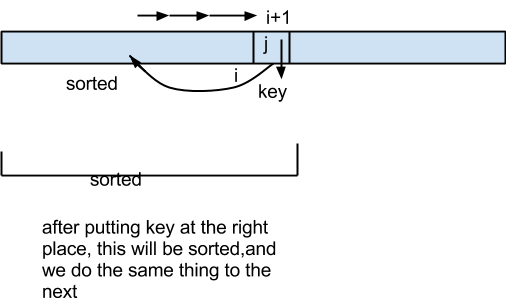
\includegraphics[scale = 0.7]{sort_insertion}\\
  \caption{Insertion sort}\label{fig.sort.insertion}
\end{figure}
8,then is what you want
2,then is what you want
3,then is what you want
4,then is what you want
ex:
\begin{verbatim}
8 2 4 9 3 6
2 8 4 9 3 6 // 2 goes before 8
2 4 8 9 3 6 // 4 goes before 8
2 4 8 9 3 6 // 9 stays there
2 3 4 8 9 6 // 3 goes before 4
2 3 4 6 8 9 // 6 goes before 8
\end{verbatim}

\begin{figure}[htbp]
  \centering
  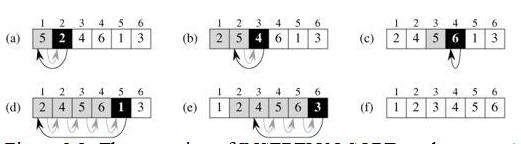
\includegraphics[scale = 0.7]{sort_insertion_example}\\
  \caption{Insertion sort}\label{fig.sort.insertion.example}
\end{figure}

python code
\begin{verbatim}
def insertionSort(L):
	#in place algorithem, 升序
	for j in range(1,len(L)):
		#将将要排序的数据保存下来, 开始对第j 个元素进行排序
		key=L[j]
		i=j-1
		#找到存放key的位置
		while i >= 0 and L[i]>key:
			L[i+1]=L[i] ## 将大数往后移动
			i=i-1
		##循环结束,说明L[i] <= key,所以key应该放在i+1处
		L[i+1]=key
	return L
\end{verbatim}

running time\\
1 already sorted: 最理想情况\\
2 reverse sorted: 最差情况

we want upper bounds 上界

kinds of analysis\\
worst-case $T(n)=$max time of any input of size n\\
average-case $T(n)=$expected time期望时间\\
(need assumption of statistical  distribution of inputs)\\
best-case (bogus假象)

BIG IDEA: \textbf{asymptotic analysis渐进分析}\\
not the the exact running time of an algorithm\\
the order of growth of the running time

the insertion sort analysis\\
worst-case: input reverse sorted
$$T(n)=\sum_{j=2}^{j=n} \theta(j)=\theta(n^2) \eqnote{算术级数arithmetic series}$$

\subsection{Merge sort}
算法\\
T(n) merge sort A[1...n]\\
$\theta(1)$	1 if n=1, done\\
$2 \times \theta(n/2)$	2 Recursively sort A[1...upper(n/2)] and A[upper(n/2)+1...n]    向上取整\\
$\theta(n)$	3 merge 2 sorted  list

Merge\\
Where is the smallest element of any two lists that are already sorted?\\
It is in one of two places, the head of the first list or the head of the second list

\textbf{Key subroutine Merge}
\begin{verbatim}
2 7 13 20
1 9 11 12
\end{verbatim}
在两个list head中,1最小,所以1是n个元素中最小的,排在最终的list的第一个位置,现在总list和两个子list成为:
\begin{verbatim}
1
2 7 13 20
9 11 12
\end{verbatim}
然后在比较两个子list 中head位置那个更小,把它放在总list的第二个位置
\begin{verbatim}
1 2
7 13 20
9 11 12
\end{verbatim}
一直这么继续下去,
这里的每一步都是固定数目的操作,和每一步中的数组的尺寸无关,每一步总,我们只关注两个head,并挑出最小的,再把数组指针推进一位,所以我知道当前的标头在哪里.
所以,对于总数为n的输入,时间是$\theta(n)$的
$遍历和排序的时间是$$\theta(n)$,有时我们称之为线性时间

merge sort的例子
\begin{figure}[htbp]
  \centering
  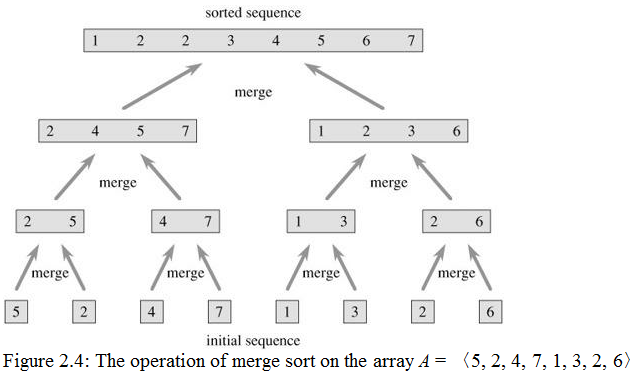
\includegraphics[scale = 0.7]{sort_merge_example}\\
  \caption{Merge sort example}\label{fig.sort.merge.example}
\end{figure}

时间复杂度
$$
T(n) =
\left\{
  \begin{array}{ll}
	\theta(1) \si n=1 \\
	2 \times T(n/2) + \theta(n) \si n>1
  \end{array}
\right.
$$

\subsection{Recursion tree}
一直做下去,得到,每一行的和都为$cn$,数的深度为$\lg n$,树的level是$\lg n+1$,最后一层的叶节点有$n$个,每一个都是$\theta(1)$

\begin{figure}[htbp]
  \centering
  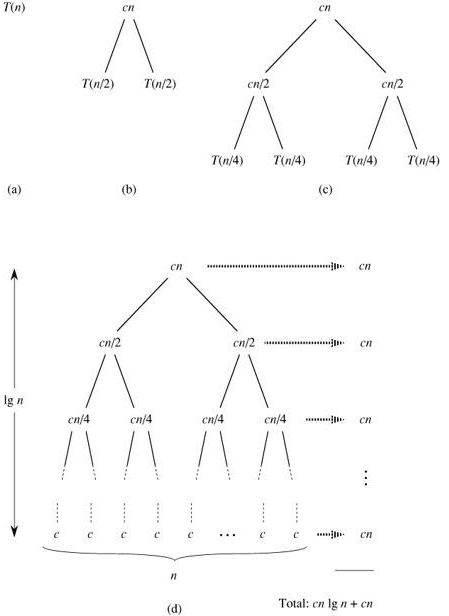
\includegraphics[scale = 0.7]{recursion_tree}\\
  \caption{Recursion tree example}\label{fig.compute.recursion_tree}
\end{figure}

为了便于计算,我们在这里设$\theta(1)=c$;
先把每一层的加起来,得到都是$cn$,然后再把所有层加起来,得到
$$T(n)=(\lg n +1)cn=\Theta(n\lg n )$$
So merge sort beats insertion sort.
$$ \theta(n\lg n )<\theta(n^2) $$

\section{渐进符号,递归及解法}
\begin{definition}
\begin{figure}[htbp]
  \centering
  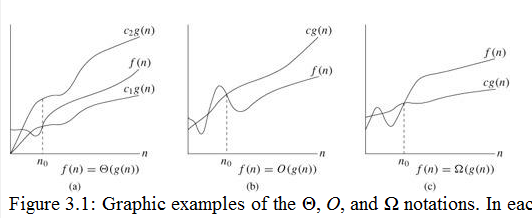
\includegraphics[scale = 0.7]{notation_asymptotical}\\
  \caption{Asymptotical notation}\label{fig.notation.asymptotical}
\end{figure}
\textbf{BIG O:上界 <=}\\
$O(g(n)) = \{f(n): $there exist positive constants $c$ and $n_0$ such that $0 \leq f(n) \leq cg(n)$ for all $n \geq n_0\}$\\
We say that $g(n)$ is an asymptotically upper bound for $f(n)$

\textbf{BIG $\Omega$下界 >=}\\
$\Omega(g(n)) = \{f(n): $there exist positive constants $c$ and $n_0$ such that $0\leq cg(n)\leq f(n)$ for all $n geq n_0\}$\\
We say that $g(n)$ is an asymptotically lower bound for $f(n)$.

\textbf{BIG $\Theta$ =}\\
$\Theta(g(n)) = \{f(n) : $there exist positive constants $c_1, c_2$, and $n_0$ such that $0\leq c\lg n\leq f(n)\leq c_2g(n)$ for all $n geq n_0\}$\\
$$\Theta(g(n))=O(g(n)) \cap \Omega(g(n)) $$\\
We say that $g(n)$ is an asymptotically tight bound for $f(n)$.

The definition of $\Theta(g(n))$ requires that every member $f(n) in \Theta(g(n))$ be asymptotically nonnegative, that is, that $f(n)$ be nonnegative whenever $n$ is sufficiently large.
\end{definition}

Ex:
$2n^2 + \Theta(n) = \Theta(n^2)$
for any function $f(n) in \Theta(n)$, there is some function $g(n) in \Theta(n^2)$ such that $2n^2 + f(n) = g(n)$ for all $n$. In other words, the right-hand side of an equation provides a coarser level of detail than the left-hand side.

o-notation
to denote an upper bound that is not asymptotically tight.\\
$o(g(n)) = \{f(n) : $for any positive constant $c > 0$, there exists a constant $n_0 > 0$ such that $0 \leq f(n) < cg(n)$ for all $n geq n_0\}$\\
For example, $2n = o(n^2)$, but $2n^2 \neq o(n^2)$

o-notation表示的是一种相差比较大的\\
in the o-notation, the function $f(n)$ becomes insignificant relative to $g(n)$ as $n$ approaches infinity; that is,
$$\lim_{n \to \infty} \frac{f(n)}{g(n)} = 0 $$

ω-notation
By analogy, ω-notation is to ?-notation as o-notation is to O-notation.
$$ \lim_{n \to \infty} \frac{f(n)}{g(n)} = \infty $$

\textbf{Comparison of functions}\\
与数的比较类比
\begin{itemize}
	\item $f(n) = O(g(n))	\approx	a \leq b$
	\item $f(n) = \Omega(g(n))	\approx a \geq b$
	\item $f(n) = \Theta(g(n))	\approx	a = b$
	\item $f(n) = o(g(n))	\approx	a \ll b$
	\item $f(n) = \omega(g(n))	\approx	a \gg b$
\end{itemize}

\subsection{Standard notations and common functions}
函数的单调性\\
monotonically increasing单调增\\
monotonically decreasing\\
strictly increasing严格递增\\
strictly decreasing

Floors and ceilings
$$
x -1 < \lfloor x \rfloor \leq x \leq \lceil x \rceil < x + 1
$$

For any integer $n, \lceil n/2 \rceil + \lfloor n/2 \rfloor = n$

And for any real number $n \geq 0$ and integer $a,b >0$
\begin{enumerate}
	\item $\lceil \lceil n/a \rceil /b \rceil = \lceil n/(ab) \rceil$
	\item $\lfloor \lfloor n/a \rfloor /b \rfloor = \lfloor n/(ab) \rfloor$
	\item $\lceil a/b \rceil \leq (a+(b-1))b$
	\item $\lfloor a/b \rfloor \geq (a-(b-1))/b$
	\item $a \mod n = a - \lfloor a/n \rfloor n$
\end{enumerate}

$\lim_{n \to \infty} \dfrac{n^b}{a^n} = 0$
from which we can conclude that
$n^b = o(a^n)$.
Thus, any exponential function with a base strictly greater than $1$ grows faster than any polynomial function.

$$
\lim_{n \to \infty} \frac{\lg ^b n}{(2^a)^{\lg n}} = \lim_{n \to \infty}\frac{\lg ^b n}{n^a} = 0
$$
$\lg^bn = o(n^a)$,
for any constant $a > 0$. Thus, any positive polynomial function grows faster than any polylogarithmic function.
$$
n! = \sqrt{2\pi n} (\frac{n}{e})^n (1 + \Theta(\frac{1}{n}))
$$
Functional iteration\\
We use the notation $f(i)(n)$ to denote the function $f(n)$ iteratively applied $i$ times to an initial value of $n$. Formally, let $f(n)$ be a function over the reals. For nonnegative integers $i$, we recursively define
$$
f^{(i)}(n) =
\left\{
  \begin{array}{ll}
		  n & \si i = 0\\
		  f(f^{(i-1)}(n)) & \si i >0
  \end{array}
\right.
$$
For example, if $f(n) = 2n$, then $f^{(i)}(n) = 2^in$.

\subsection{Substitution method}
Substitution method for solving recurrences entails two steps:\\
Guess the form of the solution.\\
Use mathematical induction(数学归纳法) to find the constants and show that the solution works.

Ex:
$T(n) = 2T(\lfloor n/2 \rfloor) + n$\\
猜测$T(n) = O(n \lg n)$,然后归纳法证明

$T(n) = 2T(n/2 + 17) + n$
与上一式相差$17$,但是当$n$很大时,$17$可以忽略掉,所以仍然猜测$T(n) = O(n \lg n)$,然后尝试用归纳法证明,发现是正确的

\subsubsection{Subtleties}
$T(n) = T(n/2) + T(n/2) + 1$.\\
我们猜测$T(n) \leq cn$\\
$T(n) \leq c n/2 + c n/2 + 1 =cn + 1$ ,wrong,但是只差了一个常数\\
we're only off by the constant 1, a lower-order term,加上一个lower-order term,猜测$T(n) \leq cn - b$\\
$T(n) \leq (c n/2 - b) + (c n/2- b) + 1 = cn - 2b + 1 \leq cn - b$\\
imply $b \geq 1$,所以当$b \geq 1$时,$T(n) \leq cn - b$

\subsubsection{Changing variables}
$T(n) = 2T(\lfloor \sqrt{n} \rfloor) +\lg n$\\
Renaming $m = \lg n$ yields  $T(2^m) = 2T(2^m/2) + m$.\\
We can now rename $S(m) = T(2^m)$ to produce the new recurrence
$S(m) = 2S(m/2) + m$,\\
这个见过,$S(m) = O(m \lg m)$.\\
Changing back from $S(m)$ to $T(n)$, we obtain
$$
T(n) = T(2^m) = S(m) = O(m \lg m) = O(\lg n \lg \lg n).
$$

\subsection{Recursion-tree method}
In a recursion tree, each node represents the cost of a single subproblem somewhere in the set of recursive function invocations.

We sum the costs within each level of the tree to obtain a set of per-level costs, and then we sum all the per-level costs to
determine the total cost of all levels of the recursion.

Recursion trees are particularly useful when the recurrence describes the running time of a divide-and-conquer algorithm.

A recursion tree is best used to generate a good guess,
which is then verified by the substitution method. So we can often tolerate a small amount of "sloppiness", since you will be verifying your guess later on.

Ex:
$T(n) = 3T(n/4) + \Theta(n^2)$\\
We create a recursion tree for the recurrence: $T(n) = 3T(n/4) + cn^2$,如图\ref{fig.compute.recursion_tree2}所示
\begin{figure}[htbp]
  \centering
  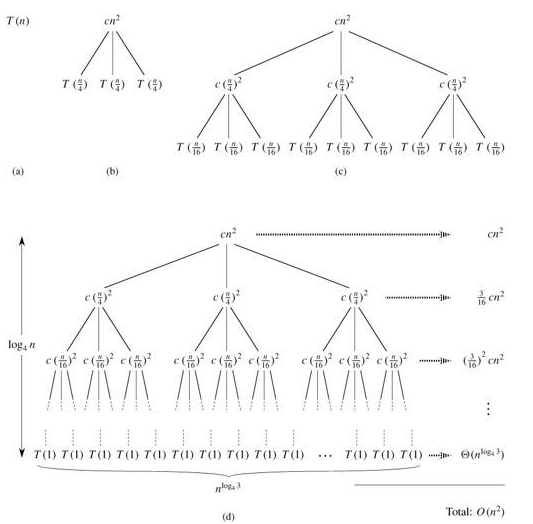
\includegraphics[scale = 0.7]{recursion_tree2}\\
  \caption{Recursion tree example}\label{fig.compute.recursion_tree2}
\end{figure}

Assume that n is an exact power of 4 (another example of tolerable sloppiness)\\
Its height is $\log_4 n$ (it has $\log_4 n + 1$ levels ($0, 1, 2,..., \log_4 n$))\\
The subproblem size for a node at depth i is $n/4^i$.\\
Each level has three times more nodes than the level above, and so the number of nodes at depth $i$ is $3i$.

深度为 $i = 0, 1, 2,..., \log_4 n - 1$,的nodes加起来 is $3^i c(n/4^i)^2 = (3/16)^icn^2$.\\
最后一层,at depth $\log_4n$, has $3^{\log_4 n} = n^{\log_4 3}$ nodes, each contributing cost $T(1)$, for a total cost of $n^{\log_4 3}T(1)$ , which is $\Theta(n^{\log_4 3})$.\\
把所有层的加起来,得到整个树的时间
\begin{equation}
\begin{split}
		T(n) & = cn^2 + \frac{3}{16} cn^2 + (\frac{3}{16})^2 cn^2 + \dots + (\frac{3}{16})^{\log_4 n - 1}cn^2 + \Theta(n^{\log_4 3}) \\
				   & = \sum_{i=0}^{\log_4 n - 1}(\frac{3}{16})^i cn^2 + \Theta(n^{\log_4 3}) \\
				   & = \frac{(3/16)^{\log_4 n} - 1}{(3/16)-1} cn^2 + \Theta(n^{\log_4 3})
\end{split}
\end{equation}
保留高阶项,得到$T(n)=O(n^2)$,
然后再用归纳法证明,发现是正确的

\subsection{Master method}
Theorem:Let $a \geq 1$ and $b > 1$ be constants, let $f(n)$ be a asymptotically positive function, and let $T(n)$ be defined on the nonnegative integers by the recurrence
$$T(n) = aT(n/b) + f(n)$$
Where we interpret $n/b$ to mean either $\lceil n/b \rceil$ or $\lfloor n/b \rfloor$. Then $T(n)$ can be bounded asymptotically as follows.
\begin{enumerate}
	\item If $f(n) = O(n^{\log_b a - \epsilon})$ for some constant $\epsilon > 0$, then $T(n) = \Theta(n^{\log_b a})$
	\item If $f(n) = n^{\log_{b} a}$, then $T(n) = \Theta(n^{\log_b a} \lg n)$
	\item If $f(n) = n^{\log_{b} a + \epsilon}$ for some constant $\epsilon > 0$, and if $a f(n/b) \leq cf(n)$ for some constant $c < 1$ and all sufficiently large $n$, then $T(n) = \Theta(f(n))$.
\end{enumerate}

总结规律如下:
Compare the function $f(n)$ with the function  $n^{\log_b a}$\\
if $f(n)$ is polynomial smaller, case $1$\\
if $f(n)$ is polynomial lager, case $3$

It is important to realize that \textbf{these three cases do not cover all the possibilities for} $f(n)$.
There is a gap between cases $1$ and $2$ when $f(n)$ is smaller than $n^{\log_b a}$ but not polynomially smaller.
Similarly, there is a gap between cases $2$ and $3$ when $f(n)$ is larger than $n^{\log_b a}$ but not polynomially larger.
If the function $f(n)$ falls into one of these gaps, or if the regularity condition in case $3$ fails to hold,
the master method cannot be used to solve the recurrence.

Ex: $T(n) = 3T(n/4) + n \lg  n$,\\
we have $a = 3, b = 4, f (n) = n \lg  n$,\\
$f(n)/(n^{\log_b a})=n\lg n/(n^{\log_4 3})=n^{1 - \log_4 3} \times \lg n$\\
so $f(n)$ is polynomial lager, case $3$, $T(n) = \Theta(n\lg  n)$.

\subsubsection{Proof of master method}
树的深度是$\log_b n$
图示证明见\ref{fig.compute.recursion_tree.proof}
\begin{figure}[htbp]
  \centering
  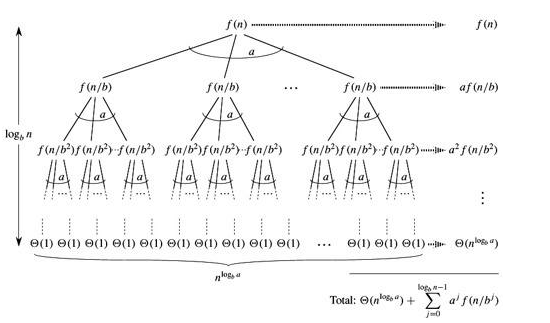
\includegraphics[scale = 0.7]{recursion_tree_proof}\\
  \caption{Recursion tree proof}\label{fig.compute.recursion_tree.proof}
\end{figure}
不太严格的证明,但是有助于理解\par
case 3:前面是呈几何级数递减的,所以前面所有层的和 is dominated by the first member $f(n)$\\
最后一层的和为$a^(\log_b n) \times  \Theta(1)=n^(\log_b a) \Theta(1)= \Theta(n^(\log_b a))$\\
$T(n)=\Theta(f(n))$\\
所以比较$f(n) and (n^(\log_b a))$也就是比较最后一层与前面所有层的

case 1:前面是呈几何级数递增的,因为$f(n)$ is polynomial smaller than $n^(\log_b a)$,所以整个求和中,$n^(\log_b a)$占据主导\\
$T(n)=\Theta(n^(\log_b a))$

case 2: 由于最顶层和最底层的差不多,在中间的,从最顶层呢过到最底层变化又不大,所以基本上都一个量级的,所以总和是:\\
$T(n)=(\log_b n+1)f(n)=(\log_b n+1) \times n^(\log_b a)=\Theta(f(n) \times \lg n)$

\section{分治法 divide and conquer}
The divide-and-conquer design paradigm
\begin{enumerate}
	\item Divide the problem (instance) into subproblems.
	\item Conquer the subproblems by solving them recursively.
	\item Combine subproblem solutions
\end{enumerate}

\subsection{Merge sort}
\begin{enumerate}
	\item Divide:Trivial.
	\item Conquer:Recursively sort 2 subarrays.
	\item Combine:Linear-time merge.
\end{enumerate}
$$
T(n)=2 \times T(n/2) +\Theta(n)=\Theta(n\lg n)
$$

\subsection{Binary serach}
find x in \textbf{sorted array}
\begin{enumerate}
	\item divide, compare x with middle
	\item conquer : recurse in one subarray
	\item combine: trivial
\end{enumerate}
$$
T(n)=\Theta(1)+1 \times T(n/2) = \Theta(\lg n)	\eqnote{master method}
$$

Algorithm $BinarySearch(L; x; first; last)$\\
Input: Array $L[first ; last]$ and value $x$.\\
Output: $1$ if $x \in L$, or $i$, $0<=  i < n$ if $L[i] = x$

pseudo code\\
if $first > last$ then return $-1$\\
else \{\\
$middle \leftarrow (first+last)/2$\\
if $L[middle]=x$ then return $middle$\\
else if $L[middle]<x$ then return $BinarySearch(L; x; middle+1; last)$\\
else return $BinarySearch(L; x; first; middle - 1)$\\
\}

\subsection{Powering a number}
given number $x$, integer $n \geq 0$, compute $x^n$\\
general method:$x \times x \times x \times x \times \cdots \times x =x^n$,  $T(n)=\Theta(n)$

Divide and conquer:
$$
x^n =
\left\{
  \begin{array}{ll}
		  x^{n/2} \times x^{n/2}  \eqnote{if n even}\\
	x^{(n-1)/2} \times x^{(n-1)/2} \times x \eqnote{if n odd}
  \end{array}
\right.
$$
$T(n)=1 \times T(n/2) +\Theta(1)=\Theta(\lg n)$\\
$T(n/2)$表示算出平方根的时间,$\Theta(1)$表示将这个算出来的平方根平方的时间

\subsection{Fibonacci numbers}
$F_0=0,F_1=1,F_2=1,F_3=3.....$\\
通式:$F_n=F_{n-1} + F_{n-2}$\\
General method: $T(n)=\Omega(\phi^n)$ with $\phi=(1+\sqrt{5})/2$
golden ratio\\
exponential time

\textbf{bottom-up}\\
Compute $F_0,F_1,F_2,....$ in order\\
当我们要计算$F_n$的时候,我们已经计算出了$F_{n-1}$ and $F_{n-2}$,直接将这两个相加,就得到$F_n$, 将两个已知数相加所需要的时间为常数\\
所以只需要依次计算各个项就可以了\\
$T(n)=n \times \Theta(1)=\Theta(n)$

\textbf{Naive recursive squaring}\\
根据Fibonacci通项公式,直接计算,and round to the nearest integer\\
但是浮点数的计算误差比较大

\textbf{Recursive squaring}
\begin{theorem}
$$
\left(
  \begin{array}{cc}
		  F_{n+1} & F_n \\
		  F_n & F_{n-1}
  \end{array}
\right)
=
\left(
  \begin{array}{cc}
		  1 & 1 \\
		  1 & 0
  \end{array}
\right)^n
$$
\end{theorem}
prove the matrix equation by induction on n
$T(n)=T(n/2)+\Theta(1)$
$T(n)=\Theta(\lg n)$

\subsection{Matrix multiplication}
input $A=a_{ij}, B=b_{ij}$\\
output $C=A \times B$\\
Standard algorithm
\begin{verbatim}
for i ←1 to n
	do for j←1 to n
			do cij←0
			for k←1 to n
				do cij←cij+ aik \times bkj
\end{verbatim}
直接计算,三层嵌套循环,时间复杂度是$\Theta(n^3)$

divide and conquer algo:\\
直接分治法
$n×n$ matrix = $2×2$ matrix of $(n/2)×(n/2)$ submatrices:

$$
\mathbf{A} =
\begin{bmatrix}
\mathbf{A}_{1,1} & \mathbf{A}_{1,2} \\
\mathbf{A}_{2,1} & \mathbf{A}_{2,2}
\end{bmatrix}
\mbox { , }
\mathbf{B} =
\begin{bmatrix}
\mathbf{B}_{1,1} & \mathbf{B}_{1,2} \\
\mathbf{B}_{2,1} & \mathbf{B}_{2,2}
\end{bmatrix}
\mbox { , }
\mathbf{C} =
\begin{bmatrix}
\mathbf{C}_{1,1} & \mathbf{C}_{1,2} \\
\mathbf{C}_{2,1} & \mathbf{C}_{2,2}
\end{bmatrix}
$$
with
$$
\mathbf{A}_{i,j}, \mathbf{B}_{i,j}, \mathbf{C}_{i,j} \in R^{2^{n-1} \times 2^{n-1}}
$$
then
$$
\begin{aligned}
\mathbf{C}_{1,1} = \mathbf{A}_{1,1} \mathbf{B}_{1,1} + \mathbf{A}_{1,2} \mathbf{B}_{2,1} \\
\mathbf{C}_{1,2} = \mathbf{A}_{1,1} \mathbf{B}_{1,2} + \mathbf{A}_{1,2} \mathbf{B}_{2,2} \\
\mathbf{C}_{2,1} = \mathbf{A}_{2,1} \mathbf{B}_{1,1} + \mathbf{A}_{2,2} \mathbf{B}_{2,1} \\
\mathbf{C}_{2,2} = \mathbf{A}_{2,1} \mathbf{B}_{1,2} + \mathbf{A}_{2,2} \mathbf{B}_{2,2}
\end{aligned}
$$
With this construction we have not reduced the number of multiplications.
We still need $8$ multiplications to calculate the $C_{i,j}$ matrices, the same number of multiplications we need when using standard matrix multiplication.

Now comes the important part. We define new matrices
$$
\begin{aligned}
& \mathbf{M}_{1} := (\mathbf{A}_{1,1} + \mathbf{A}_{2,2}) (\mathbf{B}_{1,1} + \mathbf{B}_{2,2})\\
& \mathbf{M}_{2} := (\mathbf{A}_{2,1} + \mathbf{A}_{2,2}) \mathbf{B}_{1,1}\\
& \mathbf{M}_{3} := \mathbf{A}_{1,1} (\mathbf{B}_{1,2} - \mathbf{B}_{2,2})\\
& \mathbf{M}_{4} := \mathbf{A}_{2,2} (\mathbf{B}_{2,1} - \mathbf{B}_{1,1})\\
& \mathbf{M}_{5} := (\mathbf{A}_{1,1} + \mathbf{A}_{1,2}) \mathbf{B}_{2,2}\\
& \mathbf{M}_{6} := (\mathbf{A}_{2,1} - \mathbf{A}_{1,1}) (\mathbf{B}_{1,1} + \mathbf{B}_{1,2})\\
& \mathbf{M}_{7} := (\mathbf{A}_{1,2} - \mathbf{A}_{2,2}) (\mathbf{B}_{2,1} + \mathbf{B}_{2,2})
\end{aligned}
$$
only using $7$ multiplications (one for each $M_k$) instead of $8$. We may now express the $C_{i,j}$ in terms of $M_k$, like this:
$$
\begin{aligned}
& \mathbf{C}_{1,1} = \mathbf{M}_{1} + \mathbf{M}_{4} - \mathbf{M}_{5} + \mathbf{M}_{7}\\
& \mathbf{C}_{1,2} = \mathbf{M}_{3} + \mathbf{M}_{5}\\
& \mathbf{C}_{2,1} = \mathbf{M}_{2} + \mathbf{M}_{4}\\
& \mathbf{C}_{2,2} = \mathbf{M}_{1} - \mathbf{M}_{2} + \mathbf{M}_{3} + \mathbf{M}_{6}
\end{aligned}
$$
We iterate this division process $n$ times (recursively) until the submatrices degenerate into numbers (elements of the ring $R$).
The resulting product will be padded with zeroes just like $A$ and $B$, and should be stripped of the corresponding rows and columns.

%% $$
%% \left(
%%   \begin{array}{cc}
%% 		  r & s \\
%% 		  t & u
%%   \end{array}
%% \right)
%% =
%% \left(
%%   \begin{array}{cc}
%% 		  a & b \\
%% 		  c & d
%%   \end{array}
%% \right)
%% +
%% \left(
%%   \begin{array}{cc}
%% 		  e & f \\
%% 		  g & h
%%   \end{array}
%% \right)
%% $$
%% $$
%% C = A \dot B
%% $$
%% r =ae+bg
%% s =af +bh
%% t =ce+dh
%% u =cf +dg
%% 8 multiplications of (n/2)×(n/2) submatrices
%% 4^adds of (n/2)×(n/2) submatrices
%% T(n)=8 \times T(n/2)+\Theta(n^2)
%% ($n \times n$的两个矩阵相加的时间复杂度是$\Theta(n^2)$,$n/2 \times n/2$也是$\Theta(n^2)$,与前面只是相隔了常数倍,不影响结果)
%% $n^log_b a = n^log_2 8 = n^3 ? CASE 1 ? T(n) = \Theta(n^3)$.
%% No better than the ordinary algorithm
%%
%% Strassen's algorithm
%% idea: reduce the number of multiplications
%% Multiply $2×2$ matrices with only $7$ recursive mults.
%% \begin{verbatim}
%% P1 = a ? ( f – h)
%% P2 = (a + b) ? h
%% P3 = (c + d) ? e
%% P4 = d ? (g – e)
%% P5 = (a + d) ? (e + h)
%% P6 = (b – d) ? (g + h)
%% P7 = (a – c) ? (e + f )
%%
%% r = P5 + P4 – P2 + P6
%% s = P1 + P2
%% t = P3 + P4
%% u = P5 + P1 – P3 – P7
%% \end{verbatim}
%% 7 mults, 18 adds/subs
%%
%% 我们对r进行验证一下:
%% \begin{verbatim}
%% r = P5 + P4 – P2 + P6
%% = (a + d) (e + h)
%% + d (g - e)
%% - (a + b) h
%% + (b - d) (g + h)
%% = ae + ah + de + dh
%% + dg - de
%% – ah - bh
%% + bg + bh - dg - dh
%% = ae + bg
%% \end{verbatim}

Strassen's algorithm divide and conquer
\begin{enumerate}
	\item Divide: Partition A and B into $(n/2) \times (n/2)$ submatrices. Form terms to be multiplied using $+$ and $-$, time consumed: $\Theta(n^2)$
	\item Conquer: Perform $7$ multiplications$(M1,M2, \ldots, M7)$ of $(n/2)×(n/2)$ submatrices recursively.time consumed: $7 \times T(n/2)$
	\item Combine: Form $C(r, s, t, u)$ using $+$ and $-$ on $(n/2)×(n/2)$ submatrices.time consumed: $\Theta(n^2)$
\end{enumerate}

时间复杂度
$$T(n)=7 \times T(n/2) + \Theta(n^2)=\Theta(n^{\lg7})=\Theta(n^{2.807355})$$
当前最好的为$n^{2.376}$  (理论上)

\section{快排及随机算法}
Tony Hoare在1962年发明\\
-divide and conquer\\
-sorts "in place"(merge sort needs extra space, but qsort does not)\\
-very practical(with tuning)

In the worst case, it makes $O(n^2)$ comparisons, though this behavior is rare. Quicksort is often faster in practice than other $O(n \log n)$ algorithms.\\
Additionally, quicksort's sequential and localized memory references work well with a cache.
Quicksort is a comparison sort and, in efficient implementations, is not a stable sort. Quicksort can be implemented with an in-place partitioning algorithm,
so the entire sort can be done with only $O(\log n)$ additional space used by the stack during the recursion.

Algo\\
1 Divide: partition array into $2$ sub arrays(见图\ref{fig.sort.quick.partition}) around pivot(支点) such that elements in lower $subarray<= x<=elements$ in upper subarray\\
\begin{figure}[htbp]
  \centering
  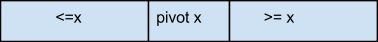
\includegraphics[scale = 0.7]{sort_quick_partition}\\
  \caption{Quick sort partition}\label{fig.sort.quick.partition}
\end{figure}
2 Conquer: recursively sort 2 subarrays\\
3 Combine: trivial(nothing to do for the combine)

\textbf{key step in quicksort is partition step}\\
快排在递归中也会进行partition\\
key: linear-time $\Theta(n)$ partitioning subroutine
\begin{verbatim}
Partition(A,p,q) //A[p...q]
x← A[p]  //pivot A[p]
i ← p
for j← p+1 to q{
    if A[j]<=x{
		i← i+1 //i加上1之后就到了大于x的那部分, 然后再将A[j] 交换到i 位置,loop invariant 保持
		exchange A[i] with A[j]
    }//end if
}//end for
exchange A[p] with A[i] // 将pivot 交换到中间, 完成partition 的任务
return i  //end function
\end{verbatim}

\begin{figure}[htbp]
  \centering
  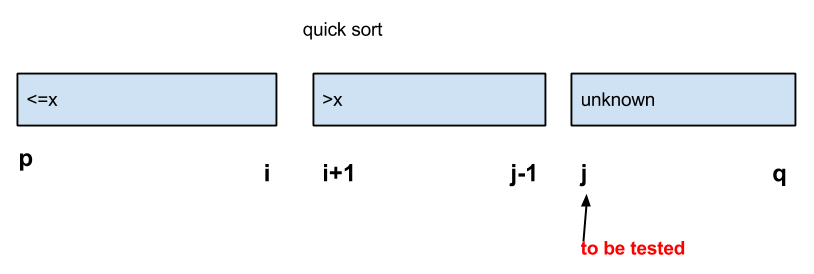
\includegraphics[scale = 0.7]{sort_quick_loopInvariant}\\
  \caption{Quick sort loop invariant}\label{fig.sort.quick.loopInvariant}
\end{figure}
At the beginning of each iteration of the loop, loop invariant
\begin{itemize}
\item if $k \in [p,i]$,then $A[k] \leq x$ and $A[p]=x$
\item if $k \in [i+1,j-1]$,then $A[k] >x$
\item if $k \in [j,q]$,then $A[k]$ unknown
\end{itemize}

running time  $T(n)\Theta(n)$  (只需要遍历一遍)
Ex: $2 8 7 1 3 5 6 4$\\
在这个例子中, 最后一个元素被选为pivot, 实际上pivot位于$p$或者$r$处都可以
\begin{figure}[htbp]
  \centering
  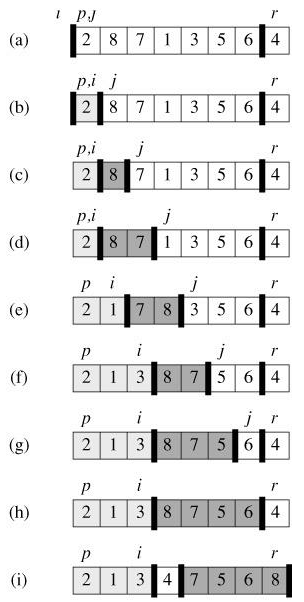
\includegraphics[scale = 0.7]{sort_quick_example}\\
  \caption{Quick sort example}\label{fig.sort.quick.example}
\end{figure}

\begin{verbatim}
Quicksort(A,p,q)
if p<q{
	r←Partition(A,p,q)
	Quicksort(A,p,r-1)
	Quicksort(A,r+1,q)
}
Initial call: Quicksort(A,1,n)
\end{verbatim}

\subsection{Analysis}
当元素数目较少时,可以换用其他更快更直接的算法,这样可以避免再简单的情况下也进行递归\\
同时,这是一个tail recursion(尾递归),所以可以使用certain tail recursion optimizations

\textbf{worst-case time}\\
-input sorted or reverse sorted 元素都被分到了一边\\
so one side of partition has no elems, the other side has $n-1$ elems\\
每次递归只减少了$1$,所以递归次数非常多\\
$T(n)
= \Theta(n)+T(0)+T(n-1)
= \Theta(n) + \Theta(1)+T(n-1)
=T(n-1) + \Theta(n)$\\
式中$\Theta(n)$表示partition所需要的时间\\
使用递归树得到时间复杂度为:$T(n)=\Theta(n^2)$

\textbf{best-case analysis(intuition only!)}\\
if we are really lucky, partition splits array $n/2:n/2$\\
$T(n)=\Theta(n)+2T(n/2)=\Theta(n\lg n)$  和merge sort一样

\textbf{Partition $1/10:9/10$}\\
$T(n)=T(n/10)+T(9n/10)+\Theta(n)$\\
用递归树得到\\
$T(n)<=(\log_{10/9}n*cn)+\Theta(n)=O(n\lg n)$\\
$T(n)<=(\log_{10}n*cn)+\Theta(n)=\Omega(n\lg n)$\\
$T(n)=\Theta(n\lg n)$\\
The reason is that any split of constant proportionality yields a recursion tree of depth $\Omega(\lg n)$ whenever the split has constant proportionality.

Suppose we alternate \textit{lucky, unlucky, lucky}...\\
$L(n)=2U(n/2)+\Theta(n)$	lucky的后面是两个unlucky\\
$U(n)=L(n-1)+\Theta(n)$	unlucky\\
Then
$$
\begin{aligned}
L(n)
&=2U(n/2)+\Theta(n) \\
&=2(L(n/2 - 1) +\Theta(n/2))+\Theta(n)\\
&=2L(n/2 - 1) + \Theta(n)\\
&=\Theta(n\lg n)  \eqnote{lucky}
\end{aligned}
$$

Suppose we alternate \textit{unlucky, lucky, unlucky, lucky}...
$$
\begin{aligned}
U(n)
&=L(n-1) + \Theta(n) \\
&=[2U((n-1)/2) + \Theta(n)] +\Theta(n)\\
&=2U((n-1)/2)) + \Theta(n)\\
&=2U(n/2) + \Theta(n)\\
&=\Theta(n\lg n)  \eqnote{lucky}
\end{aligned}
$$

So when we alternate lucky, unlucky, lucky...,we are lucky\\
Or we alternate unlucky, lucky, unlucky, lucky..., we are luck too.\\
So how do we ensure that we are usually lucky? \\
Because if the input is already sorted or reverse sorted, we are going to be unlucky.\\
1.randomly arrange the elements\\
2.randomly choose the pivot

\subsection{Random quicksort}
pick the pivot randomly\\
选择好之后,把这个选中的与array的第一个元素交换位置,这样这个随机选择的pivot就到了array的第一位置,然后再运行Partition函数
\begin{itemize}
\item 运行时间不取决于输入数据的顺序
\item 对输入序列的分布不用做出假设
\item 不存在特定的输入序列会引起worst-case
\item worst-case determined only by random number generator
\end{itemize}

\subsection{Median-of-3 Pivot}
For example, the median-of-3 pivot approach selects three candidate pivots and uses the median one.
If the three pivots are chosen from the first, middle and last positions, then it is easy to see that for the already sorted array,
this will produce an optimum result: each partition will be exactly half ($\pm$ one element) of the problem and we will need exactly ceiling($\log n$) recursive calls.

\subsection{Random method analysis}
Random variable(随机变量) for running time assuming that random numbers are independent.\\
I want to know where I pivoted. 设这个pivot 的位置为随机变量$k$\\
So for $k=0, 1...n-1$ let\\
$x_k=1$ if partition generates a $k: n-k-1$ split, (pivot 算一个数, 所以两者加起来是n-1)\\
$x_k=0$ otherwise\\
这样一个partition,就产生了$n$个random variable,其中只有一个是$1$,其余的都是$0$.\\
例如如果产生的partition为$5:n-6$,那么只有$x_5=1,x_i=0 (i \in  [[0,n-1]]$ and $i!=5)$\\
this type of random variable is called \textbf{indicator random variable}

the expected value of $x_k:\\
E[x_k]=0*P(x_k =0)+1*P(x_k =1) = P(x_k =1) =1/n$\\
因为每一个数$k$ 都有可能取到, 而且概率是一样的, 所以每个数的概率都是 $1/n$
$$
T(n) =
\left\{
  \begin{array}{ll}
		  T(0) + T(n-1) \si 0:n-1 split \\
		  T(1) + T(n-2) \si 1:n-2 split \\
            \vdots \\
		  T(n-1) + T(0) \si n-1:0 split
  \end{array}
\right.
$$
所以这就是T(n)的递归,但是这个递归很麻烦,这里我们就可以看到indicator random variable的优美性,我们将使用indicator random variable将这个递归reduce to(规约到数学上)
$$
T(n) = \sum_{k=0}^{n-1} x_k (T(k) + T(n-k-1) + \Theta(n))
$$

$T(n)$的期望
\begin{equation}
\begin{split}
   E[T(n)] & =E[\sum_{k=0}^{n-1}x_k(T(k)+T(n-k-1)+\Theta(n))] \\
           & =\sum_{k=0}^{n-1}E[x_k(T(k)+T(n-k-1)+\Theta(n))]\\
           & \text{$x_k$随机变量独立于任何其他的partitions, 也就是说$x_k$ 区别于}\\
           & \text{其他递归调用,所以积的期望等于期望的积}\\
           & =\sum_{k=0}^{n-1}E[x_k]*E[(T(k)+T(n-k-1)+\Theta(n))]\\
           & = \frac{1}{n}\sum_{k=0}^{n-1}E[(T(k)] + \frac{1}{n}\sum_{k=0}^{n-1}E[T(n-k-1)] +\frac{1}{n}\sum_{k=0}^{n-1}\Theta(n)\\
           & =\frac{2}{n}\sum_{k=0}^{n-1}E[(T(k)] +\Theta(n)
\end{split}
\end{equation}

$x_k$ 是对$n$进行partition时产生的一个indicator random variable也就是说$x_k$是和$T(n)$ 是相关的, 而后面的$T(k)$ 与$T(n-k-1)$是在有了$x_k$ 之后, 也就是产生了一个$k,n-k-1$的分割后, 对产生的两个新的分割求时间时, 又会产生新的indicator: $x'_k$\\
所以$x_k$ 与$T(k), T(n-k-1)$是相互独立的, 可以运用概率的乘法原则

Absorb $k=0,1$ terms into $\Theta(n)$ for tech convenence,(两个常量加进去不影响$\Theta(n)$)
$$
E[T(n)]=\frac{2}{n}\sum_{k=2}^{n-1}E[T(k)]+\Theta(n)
$$

Use fact\todo{how to prove?}
$$
\sum_{k=2}^{n-1}k\lg k \leq \frac{1}{2}n^2\lg n-\frac{1}{8}n^2
$$
To prove $E[T(n)]<=a*n\lg n$ for constant $a>0$ with the substitution method\\
$E[T(n)] \leq an \lg n –bn (a, b >0)$\\
.....\\
所以我们得到$T(n)$的期望值是$\Theta(n\lg n)$\\
so the running time of randomized quicksort is $\Theta(n\lg n)$

The version of PARTITION given in this chapter is not the original partitioning algorithm. Here is the original partition algorithm, which is due to T.Hoare:
\begin{verbatim}
HOARE-PARTITION(A, p, r)
 1  x ← A[p]
 2  i ← p - 1
 3  j ← r + 1
 4  while TRUE
 5      do repeat j ← j - 1
 6           until A[j] <= x
 7         repeat i ← i + 1
 8           until A[i] >= x
 9         if i < j
10            then exchange A[i] with A[j]
11            else return j
\end{verbatim}
Every element of $A[p ‥ j]$ is less than or equal to every element of $A[j +1 ‥ r]$ when HOARE-PARTITION terminates.\\
The HOARE-PARTITION procedure always places the pivot value (originally in $A[p]$) into one of the two partitions $A[p ‥ j]$ and $A[j + 1 ‥ r]$.

\subsection{Exercise}
[Exercises 7.4-5]
The running time of quicksort can be improved in practice by taking advantage of the fast running time of insertion sort when its input is "nearly" sorted.
When quicksort is called on a subarray with fewer than $k$ elements, let it simply return without sorting the subarray.
After the top-level call to quicksort returns, run insertion sort on the entire array to finish the sorting process.
Argue that this sorting algorithm runs in $O(nk + n \lg(n/k))$ expected time. How should k be picked, both in theory and in practice?

[Problems 7-6: Fuzzy sorting of intervals]
Consider a sorting problem in which the numbers are not known exactly. Instead, for each number, we know an interval on the real line to which it belongs.
That is, we are given n closed intervals of the form $[a_i, b_i]$, where $a_i \leq b_i$.
The goal is to fuzzy-sort these intervals, i.e.,to produce a permutation $〈i_1, i_2,\ldots, i_n〉$ of the intervals such that for $j = 1,2,\ldots,n$
there exist $c_j \in [a_{i_j}, b_{i_j}]$, satisfying $c_1 \leq c_2 \leq \cdots \leq c_n$.\\
1.	Design an algorithm for fuzzy-sorting $n$ intervals. Your algorithm should have the general structure of an algorithm that
quicksorts the left endpoints (the $a_i$ values), but it should take advantage of overlapping intervals to improve the running time.
(As the intervals overlap more and more, the problem of fuzzy-sorting the intervals gets easier and easier.
Your algorithm should take advantage of such overlapping, to the extent that it exists.)\\
2.	Argue that your algorithm runs in expected time $\Theta(n \lg n)$ in general, but runs in expected time $\Theta(n)$
when all of the intervals overlap (i.e., when there exists a value $x$ such that $x \in [a_i, b_i]$ for all $i$).
Your algorithm should not be checking for this case explicitly; rather, its performance should naturally improve as the amount of overlap increases.

\section{Heapsort}
Implementation of heap: tree or array\\
Max-heap: parent $\geq$ children,
	heapsort\\
Min-heap: parent $\leq$ children,
	priority queue

下面我们以Max-heap 进行讲解\\
Array n elements, leaves: $floor(n/2) + 1, floor(n/2) + 2, floor(n/2) + 3, \cdots, n$

The (binary) heap data structure is an array object that we can view as a nearly complete binary tree
\begin{verbatim}
PARENT(i)
   return floor(i/2)
LEFT(i)
   return 2i
RIGHT(i)
   return 2i + 1
\end{verbatim}

\begin{figure}[htbp]
  \centering
  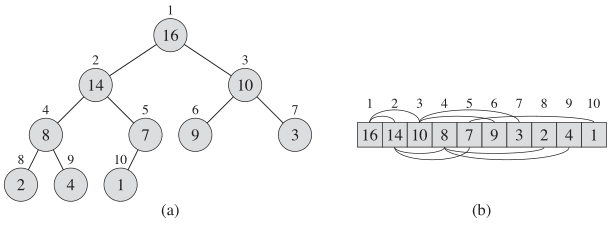
\includegraphics[scale = 0.7]{sort_heap_example}
  \caption{An example of heap}\label{fig.sort.heap.example}
\end{figure}

The height of a node: the length of the longest downward path to a leaf from that node\\
The depth of a node: the length of the path to its root\\
Root node has depth 0, leaf node has height 0

\subsection{Maintaining the heap property}
Its inputs are an array A and an index i into the array\\
A[i] "float down"

\begin{verbatim}
Max-heapify(A, i)
   l = left(i)
   r = right(i)
   if l <= A.heap-size and A[l] > A[i]
      largest = l
   else largest = i
   if r <= A.heap-size and A[r] > A[i]
      largest = r
   if largest != i
      exchange A[i] with A[largest]
      Max-heapify(A, largest)
\end{verbatim}

max heapify: correct a single violation of the heap property in a sub tree's root\\
\textbf{运行Max-heapify(A, i) 的前提条件precondition}: assume that the trees rooted at left(i) and right(i) are max-heaps

\begin{figure}[htbp]
  \centering
  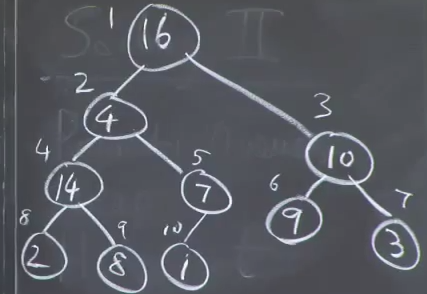
\includegraphics[scale = 0.7]{sort_heap_violation}
  \caption{An example of violation of heap property}\label{fig.sort.heap.violation}
\end{figure}
图\ref{fig.sort.heap.violation}中的第二个节点violates the max heap property, 所以我们可以调用max-heapify(A, 2), 修复好这个之后, 再进行检查直到不出现violation 为止

The children's subtrees each have size at most $2n/3$\todo{not understood}—the worst case occurs when the bottom level of the tree is exactly half full—and therefore we can describe the running time of MAX-HEAPIFY by the recurrence\\
$T(n) \leq T(2n/3) +\Theta(1)$\\
master theorem => $T(n) = O(\lg n)$

add a new item : place the new item at the last position(向左向下走知道不能继续前进), 然后进行修复, compare it with its parent, if it is larger than its parent, exchange them 向上继续进行这个比较直到不违反heap的性质, 也就是向上修复\\
delete the root : 将最后一个节点的值赋给root, 然后向下进行修复

\subsection{Building a heap}
build-max heap: produce a max heap from an unordered array

The elements in the subarray $A[(floor(n/2)+ 1)…n]$ are all leaves of the tree\todo{how to prove}\\
而leaf 已经是max-heap了, 因为leaf 没有children

The procedure BUILD-MAX-HEAP goes through the remaining nodes of the tree and runs MAX-HEAPIFY on each one
\begin{verbatim}
Build-Max-heap(A)
A.heap-size = A.length
    for i = floor(A.length / 2) downto 1
        Max-heapify(A, i) //每次调用max-heapify 之前, 都是满足max-heapify的precondition的
\end{verbatim}

Each call to MAX-HEAPIFY costs $O(\lg n)$ time, and BUILD-MAX-HEAP makes $O(n)$ such calls. Thus, the running time is $O(n\lg n )$. This upper bound, though correct, is not asymptotically tight.

但是我们可以发现:\\
max-heapify takes $O(1)$ for nodes that are one level above the leaves\\
and in general $O(l)$ time for nodes that re l levels above the leaves

an n-element heap has height $floor(\lg n )$ and at most $ceil(n/(2^{h+1}))$ nodes of any height $h$\todo{need proof}

$$
\sum_{h=0}^{\lfloor \lg n \rfloor} \lceil \frac{n}{2^{h+1}} \rceil O(h)
=
O(n \sum_{h=0}^{\lfloor \lg n \rfloor} \frac{h}{2^h})
$$

$$
\sum_{h=0}^{\infty} \frac{ h}{2^h} = \frac{1/2}{(1 - 1/2)^2} = 2
$$
Thus, we can bound the running time of BUILD-MAX-HEAP as
$$
O(n \sum_{h=0}^{\lfloor \lg n \rfloor} \frac{h}{2^h})
= O(n \sum_{h=0}^{\infty} \frac{h}{2^h})
= O(n)
$$

Hence, we can build a max-heap from an unordered array in linear time

\subsection{The heapsort algorithm}
build-max-heap from unordered array\\
find max element $A[1]$\\
swap elements $A[n]$ with $A[1]$, now max element is at the end of the array\\
Discard node $n$ from heap,\\
New root may violate max heap property, fix it

\begin{verbatim}
Heapsort(A)
    Build-Max-heap(A)
    for i = A.length downto 2
        exchange A[1] with A[i]
        A.heap-size = A.heap-size - 1
        Max-heapify(A, 1)
\end{verbatim}

把$A[1]$ 也就是最大值挪到最后一个位置, 同时将heap 的大小减一, 这样最大值就从heap 从取出来了并被放在了正确的位置上, 然后再修复这个heap; 然后再最大值重复这个操作

time $O(n\lg n )$\\
in place sort

\subsection{Priority queues}
max-priority queue, min-priority queue\\
we can use a heap to implement a priority queue

\begin{verbatim}
HEAP-MAXIMUM(A)
    return A[1]
\end{verbatim}
heap-maximum: $\Theta(1)$ time

\begin{verbatim}
HEAP-extract-MAX(A)
    if A.heap-size < 1
        error "heap underflow"
    max = A[1]
    A[1] = A[A.heap-size]
    A.heap-size = A.heap-size - 1
    MAX-HEAPIFY(A,1)
    return max
\end{verbatim}
heap-extract-max: $O(\lg n )$ time

\begin{verbatim}
HEAP-INCREASE-KEY(A,i,key)
    if key < A[i]
        error "new key is smaller than current key"
    A[i] = key
    while i > 1 and A[PARENT(i)] < A[i]
        exchange A[i] with A[PARENT(i)]
        i = PARENT(i)
\end{verbatim}
HEAP-INCREASE-KEY: $O(\lg n )$ time

\begin{verbatim}
MAX-HEAP-INSERT(A,key)
    A.heap-size = A.heap-size + 1
    A[A.heap-size] = -\infty
    HEAP-INCREASE-KEY(A,A.heap-size,key)
\end{verbatim}
MAX-HEAP-INSERT: $O(\lg n )$ time

\section{线性时间排序}
\begin{itemize}
\item quicksort $\Theta(n\lg n )$  randomized
\item heapsort $\Theta(n\lg n )$ 堆排序
\item merge sort $\Theta(n\lg n )$
\item insertion sort $\Theta(n^2)$
\end{itemize}

can we do better than $\Theta(n\lg n )$?\\
comparison sorting model\\
only use comparisons to determine relative order of elements

\subsection{decision tree model 决策树}
Ex: sort $<a_1, a_2, a_3>$

In general $<a_1,a_2...,a_n>$
\begin{itemize}
\item each internal node labeled $i, j$ means compare $a_i$ vs. $a_j$
\item left subtree $a_i <= a_j$
\item right subtree $a_i > a_j$
\item each leaf gives a permutation of the array
\end{itemize}

图\ref{fig.decision_tree.example}是一个决策树的例子
\begin{figure}[htbp]
  \centering
  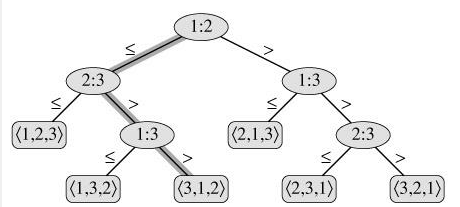
\includegraphics[scale = 0.7]{decision_tree_example}\\
  \caption{Decision tree example}\label{fig.decision_tree.example}
\end{figure}

\textbf{A lower bound for the worst case}\\
The length of the longest path from the root of a decision tree to any of its reachable leaves represents the worst-case number of comparisons. Consequently,
the worst-case number of comparisons for a given comparison sort algorithm equals the height of its decision tree. A lower bound on the heights of all decision trees in which each permutation appears as a reachable leaf is therefore a lower bound on the running time of any comparison sort algorithm. The following theorem establishes such a lower bound.

[Theorem 8.1] Any comparison sort algorithm requires $\Omega(n \lg n)$ comparisons in the worst case.\\
Proof: From the preceding discussion, it suffices to determine the height of a decision tree in which each permutation appears as a reachable leaf.\\
Consider a decision tree of height h with l reachable leaves corresponding to a comparison sort on n elements.
Because each of the $n!$ permutations of the input appears as some leaf, we have $n! \leq l$.(至少含有$n!$ 个leaves)
Since a binary tree of height h has no more than $2^h$ leaves, we have\\
$n! \leq l \leq 2^h$,
which, by taking logarithms, implies\\
$h \geq \lg (n!) = \Omega(n\lg n)$ (Stirling's approximation $n! \simeq (n/e)^n$

\subsection{Counting sort计数排序}
Element $\in [0, k]$ for some integer $k$. \\
When $k = O(n)$, the sort runs in $\Theta(n)$ time.\\
The \textbf{basic idea} of counting sort is to \textbf{determine, for each input element $x$, the number of elements less than $x$}.
This information can be used to place element $x$ directly into its position in the output array.\\
For example, if there are $17$ elements less than $x$, then $x$ belongs in output position $18$.
This scheme must be modified slightly to handle the situation in which several elements have the same value,
since we don't want to put them all in the same position.

input array $A[1,\ldots, n]$, and thus $length[A] = n$.\\
the array $B[1,\ldots,n]$ holds the sorted output, \\
the array $C[0,\ldots,k]$ provides temporary working storage.

\begin{verbatim}
COUNTING-SORT(A, B, k)
 1  for i ← 0 to k
 2     do C[i] ← 0
 3  for j ← 1 to length[A]
 4     do C[A[j]] ← C[A[j]] + 1
 5  // C[i] now contains the number of elements equal to i.
 6  for i ← 1 to k
 7     do C[i] ← C[i] + C[i - 1]
 8  // C[i] now contains the number of elements leqi
 9  for j ← length[A] downto 1
10     do B[C[A[j]]] ← A[j]
11        C[A[j]] ← C[A[j]] - 1
\end{verbatim}

An important property of counting sort is that it is \textbf{stable}.

Analysis\\
line $1-2 \Theta(k)$\\
line $3-4 \Theta(n)$\\
line $6-7 \Theta(k)$\\
line $9-11 \Theta(n)$\\
Overall time$\Theta(n+k)$\\
在实际上, 当 $k\Theta(n)$ 时, 我们才采用 counting sort

[Exercises 8.2-3] Suppose that the for loop header in line $9$ of the COUNTING-SORT procedure is rewritten as
\begin{verbatim}
9	 for j ← 1 to length[A]
\end{verbatim}
Show that the algorithm still works properly. Is the modified algorithm stable?\\
凭直觉来看, 不是stable

\subsection{Radix sort基数排序}
LSD(Least Significant Digit first)的基数排序适用于位数小的数列,如果位数多的话,使用MSD的效率会比较好.\\
MSD(Most Significant Digit first)的方式与LSD相反,是由高位数为基底开始进行分配,但在分配之后并不马上合并回一个数组中,
而是\textbf{在每个"桶子"中建立"子桶"},将每个桶子中的数值按照下一数位的值分配到"子桶"中.在进行完最低位数的分配后再合并回单一的数组中.

这里讲到的是LSD

\subsubsection{说明}
其原理在于对于待排序的数据,\textbf{整体权重未知}的情况下,
先按权重小的因子排序,然后按权重大的因子排序.\\
例如比较时间,先按日排序,再按月排序,最后按年排序,仅需排序三次.

但是如果先排序高位就没这么简单了.\\
\textbf{基数排序源于老式穿孔机,排序器每次只能看到一个列(这就是一个整体权重未知的例子)},
很多教科书上的基数排序都是对数值排序(这样意义不大),数值的大小是已知的,与老式穿孔机不同.将数值按位拆分再排序,是无聊并自找麻烦的事.算法的目的是找到最佳解决问题的方案,而不是把简单的事搞的更复杂.

\textbf{基数排序更适合用于对时间,字符串等这些整体权值未知的数据进行排序.}
这时候基数排序的思想才能体现出来,例如字符串,如果从高位(第一位)往后排就很麻烦.
而反过来,先对影响力较小,的低位(最后一位)进行排序就非常简单了.
这时候基数排序的思想就能体现出来.

$d$ 位数字, 每一位数字可以取 $k$ 个不同的数, 例如$0$ 到$9$ 十个数, 那么$k=10$
\begin{verbatim}
RADIX-SORT(A, d)
    for i from 1 to d:
        do use a stable sort to sort array A on digit i
\end{verbatim}

\subsubsection{Analysis}
time:$\Theta(d(n+k))$

证明:correctness\\
induct on digit position $t$\\
assume by induction 前$t-1$位已经排好序, 我们需要对第$t$位进行排序\\
1, if two elements have same t\textsuperscript{th} digit, stability $\Rightarrow$ same order $\Rightarrow$ sorted order\\
2, if different t\textsuperscript{th} digit $\Rightarrow$ sorted order

---use counting sort digits\\
---suppose we have $n$ integers each $b$ bits ( $range=[0,2^b-1]$, non-negative)\\
---split into $b/r$ "digits" each $r$ bits (将$r$个bits组合成一个大的"bit")\\
time $O(b/r*(n+k))=O(b/r*(n+2^r))$\\
对r求导, 令其为零求得此时的r值 $r=\lg n$\\
得到$O(bn/\lg n )$

if number in range $0,2^b-1$ then $time = O(dn)$\\
if  $d=O(1)$ then $time=O(n)$

而且只要$d$小于$\lg n$, 就可以击败comparison sort\\
但是在实际上, counting sort is not very good on a cache, in practice, radix sort is not that fast, unless your numbers are really small.\\
但是在理论上, 这个算法很优美

Finally, if you have arbitrary integers, that are one word length long, and you can manipulate a word in constant time.\\
Then the best algorithm we known for sorting runs $n*\sqrt{\lg\lg n }$, and this is a randomized algorithm and very complicated\\
有另外一个算法$n*lg(\lg n )$ worst case, 这篇论文应该可以看懂

\section{Order statistics}
given n elements\\
find $k$th smallest element\\
naive algorithm: sort and return $A[k]$\\
$k=1$ minimum\\
$k=n$ maximum\\
median 中位数 $k=floor((n+1)/2)$ or $ceil((n+1)/2)$

randomized divide and conquer\\
random-select \\
$\Theta(n)$ expected running time\\
$\Theta(n^2)$ worst-case  差不多是$1/n^n$ 的概率\\
intuition for analysis\\
(we assume 所有数都不等)\\
lucky case: $1/10, 9/10$\\
$T(n) \leq T(9/10n)\Theta(n)$  假设第$i$小的位于$9/10$部分\\
unlucky case: $0, n-1$\\
$T(n)=T(n-1)\Theta(n)\Theta(n^2)$

indicator random variable\\
let $T(n)$  be the random variable for running time of random-select\\
define indicator random variable $x_k, k \in [0, n-1]$\\
$x_k = 1$	if partition generates an $k$ to $n-k-1$ splits \\
$x_k = 0$	otherwise

substitution method , $E[T(n)] \leq cn$\\
$3/8n^2$ induction to get $3/8$

worst-case linear time order statistics

Why do we group in $5$ numbers, not $3$ or $7$ or others?\\
$3$是不行的, $7$也行, 但是对于效率没有什么提升

\section{Hashing}
symbol-table problem in compiler\\
table S holding n symbols\\
\textbf{dictionary operations}\\
inset(S, x) x is an element\\
delete(S, x)\\
search(S, k) for a given key\\
search time $\Theta(n)$ in the worst case\\
search time $\Theta(1)$ the expected time\\

\subsection{Direct address tables}
Direct addressing is applicable when we can afford to allocate an array that has one position for every possible key.

\begin{verbatim}
Direct-address-search(T, k)
    return T[k]

Direct-address-insert(T, x)
    T[key[x]] =x

Direct-address-delete(T, x)
    T[key[x]] =nil
\end{verbatim}

\subsection{Hash tables}
With direct addressing, an element with key k is stored in slot $k$.\\
With hashing, this element is stored in slot $h(k)$; that is we use a \textbf{hash function} $h$ to compute the slot from the key $k$.\\
Here $h$ maps the universe $U$ of keys into the slots of a \textbf{hash table} $T[0,\ldots, m-1]$\\
$h: U \rightarrow {0,1, \ldots m-1}$

\paragraph{collision: two keys hash to the same slot.}~\\
Solution: make h appear random thus avoiding collisions or at least minimizing their number.\\
Since $|U|>m$, 肯定会有collisions

\paragraph{Collision resolution by chaining}~\\
We put all elements that hash to the same slot in a linked list.\\
Slot $j$ contains a pointer to the head of list of all stored elements that hash to $j$.\\
通过这种方式解决collision的dictionary operations很容易实现

\begin{verbatim}
chain-hash-insert(T, x)
    insert x at the head of list T[h(key[x])]

chain-hash-search(T, k)
    search for an element with key k in list T[h(k)]

chain-hash-delete(T, x)
    delete x from the list T[h(key[x])]
\end{verbatim}

\paragraph{Analysis}~\\
Insert: worst-case $O(1)$\\
插入很快, 是因为我们假设hash table之前不含有x; 当然我们可以在insert之前先search一遍\\
Search: proportional to the length of linked list\\
Delete: $O(1)$ if the list is doubly linked\\
	same as search if the list is singly linked

\textit{How well does hashing with chaining perform? In particular, how long does it take to search for an element with a given key?}\\
Def.: the \textbf{load factor} of a hash table with n keys and m slots is\\
$\alpha = n/m =$average keys in a slot$=$ average number of elements stored in a chain

\textbf{worst-case}\\
集合S中的所有键经过hash函数生成的hash值是一样的, 因此all elements go to the same slot\\
the access time is $\Theta(n) + $the time to compute the hash function.

\textbf{average-case}\\
assumption of \textbf{simple uniform hashing}\\
---any given element is equally likely to hash into any of the m slots, independently of where any other element has hashed to.

For $i \in [0,m-1]$, let us denote $n_i$ the length of the list $T[i]$\\
So that $n=n_0 + n_1 + \ldots + n_{m-1}$\\
And the average value of $n_i$ is $E[n_i]=\alpha=n/m$

expected unsuccessful search time $\Theta(1+n/m)$  其中1是指进行hash操作的时间\\
expected successful search $time =\Theta(1+n/m)$

Page $227$: \todo{为什么是成比例的, 搜索哪个list不是通过计算key的hash值来确定的吗?}the situation for a successful search is slightly different, since each list is not equally likely to be searched. Instead, \red{the probability that a list is searched is proportional to the number of elements it contains}. Nonetheless, the expected search time is still $\Theta(1+\alpha)$\par
Proof: the number of elements examined during a successful search for an element $x$ is $1$ plus the number of elements that appear before $x$ in x's list. Elements before $x$ in the list were all inserted after $x$ was inserted.\\
Let $x_i$ denote the i\textsuperscript{th} element inserted into the table, and let $k_i=key[x_i]$\\
For keys $k_i$ and $k_j$ ($k_j$注意细微差别), \\
we define indicator random variable $X_{ij}=I{h(k_i)=h(k_j)}$\\
Under the assumption of simple uniform hashing, we have $Pr\{h(k_i)=h(k_j)\}=1/m$\todo{how to compute?}\\
$So E[X_{ij}]=1/m$\\
For $x_i$, the number of elements examined in a successful search is $(1+\sum_{j=i+1}^n X_{ij})$, 其中的$1$是$x_i$ 本身, 他自己也要被检查\\
Thus, the expected number of elements examined in a successful search is:
$$
E[\frac{1}{n} \sum_{i=1}^n (1 + \sum_{j = i + 1}^n X_{ij})]
= 1 + \frac{n-1}{2m}
= 1 + \frac{\alpha}{2} - \frac{\alpha}{2n}
$$

Thus the total time required for a successful search(including the time for computing the hash function) is $\Theta(2 + \alpha/2 - \alpha/{2n}=\Theta(1+\alpha)$

if that is to say When the number of hash-table slots is at least proportional to the number of elements in the table, that is to say $n\Theta(m)$ and $ \alpha \Theta(1)$. Thus searching takes constant time on average. \\
Since insertion takes $O(1)$ worst-case time and deletion takes $O(1)$ worst-case time when the lists are doubly linked, all dictionary operations can be supported in $O(1)$ time on average.

\subsection{Hash functions}
A good hash function satisfies (approximately) the assumption of simple uniform hashing.\\
但是我们很少能够知道keys的distribution, 所以这个条件很难满足.\\
如果我们知道distribution, 例如, if the keys are known to be random real numbers k independently and uniformly distributed in the range $0<=k<1$, the hash function\\
$h(k) = floor(km)$ 满足simple uniform hashing的条件.

In practice, heuristic(启发式的) techniques can often be used to create a good hash function.

\underline{Interpreting keys into natural numbers}:\\
Most hash functions assume that the universe of keys is the set $N={0,1,2, \ldots}$ of natural numbers\\
因此, 当keys不是自然数时, 需要将其转化为自然数.\\
例如, a character string $\rightarrow$ natural number \textbf{in suitable radix notation}\\
For example: the string pt, $(112, 116)$ in ASCII character set, then expressed as a radix$-128$\todo{to be checked} integer, pt becomes $112*128+116=14452$

\subsubsection{Division method}
$h(k)=k \mod m$\\
When using the division method, we usually avoid certain values of $m$.\\
\red{一个数对$2^r$取余, 结果就是这个数的二进制表示的最后$r$位数字\\
同样的道理, 一个数对$10^r$取余, 结果就是这个数 的$10$进制表示的最后$r$位数字}\\
所以选择一个质数来作为$m$比较好, 这个质数一定不要接近$2$或者$10$的某个指数

\subsubsection{Multiplication method}
$h(k)=floor(m(kA\mod 1))$\\
where $x \mod 1$ mans the fractional part of $x$, that is $x - floor(x)$\\
$A$ is constant $\in (0,1)$

An advantage of the multiplication method is that the value of m is not critical. We typically choose it to be a power of $2$($m=2^p$ for some integer $p$). 这样multiplication method 就很容易在计算机上实现

\underline{具体执行方法}\\
word size of the machine: $w$ bits\\
$k$ fits into a single word\\
A is a fraction of the form $s/2^w$, where s is an integer in the range $0 < s < 2^w$. \\
we first multiply $k$ by the $w$-bit integer $s = A \cdot 2^w$. The result is a $2w$-bit value $r1*2^w + r0$, where $r1$ is the high-order word of the product and $r0$ is the low-order word of the product. \\
The desired $p$-bit hash value consists of the $p$ most significant bits of $r0$.\\
%% 这里有一个图片figure :D:\my-container\Documents\算法导论\figure\hash_multiplication_method.png\\
\begin{figure}[htbp]
  \centering
  % Requires \usepackage{graphicx}
  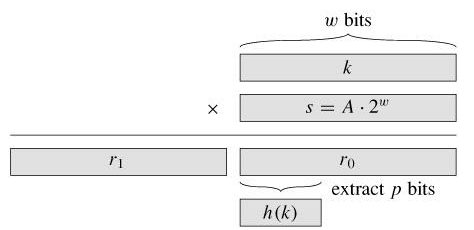
\includegraphics[width= 0.5\textwidth]{hash_multiplication_method}\\
  \caption{Multiplication method for Hash}\label{fig.hash.mult}
\end{figure}

Although this method works with any value of the constant A, it works better with some values than with others.\\
$A=(\sqrt{5} - 1)/2=0.6180339887$

\underline{Example}: suppose we have $k = 123456, p = 14, m = 2^{14} = 16384$, and $w = 32$. Adapting Knuth's suggestion, we choose $A$ to be the fraction of the form $s/232$ that is closest to , so that $A = 2654435769/232$. \\
Then $k \times s = 327706022297664 = (76300 \times 2^{32}) + 17612864$, \\
and so $r1 = 76300$ and $r0 = 17612864$\\
The $14$ most significant bits of $r0$ yield the value $h(k) = 67$\todo{14bits为什么只有67, 这么小??? 不知道这个是怎么算出来的}.\\
$17612864$的二进制表示为: $1000, 0110, 0110, 0000, 0010, 0000, 0$\\
$m=2^p$ and word size of machine is $w$-bit, \\
$k$ fits into a singl word\\
$h(k)=(A*k\mod 2^w) rsh (w-r)$\todo{这个是MIT视频教程中使用的方法}\\
A an odd integer in the range $(2^{w-r}-1, 2^w)$, don't pick $A$ too close to $2^{m-1}$ or $2^w$\\
rsh right shift

\subsubsection{Collision resolution by open addressing}
all elements are stored in the hash table itself.\\
-- no storage for links

进行多次hash操作直到找到一个空的slot\\
probe sequence should be a permutation

table may full up $\mathbf{n \leq m}$\\
deletion is difficult

\todo{这一段没有怎么看懂. 书上的237页}To perform insertion using open addressing, we successively examine, or probe, the hash table until we find an empty slot in which to put the key. Instead of being fixed in the order $0, 1, \ldots, m - 1$ (which requires $\Theta(n)$ search time), the sequence of positions probed depends upon the key being inserted. To determine which slots to probe, we extend the hash function to include the probe number (starting from $0$) as a second input. Thus, the hash function becomes\\
$h : U \times {0, 1, \ldots, m - 1} \rightarrow {0, 1, \ldots, m - 1}$.\\
With open addressing, we require that for every key $k$, the probe sequence\\
$〈h(k,0),h(k,1), \ldots, h(k,m - 1)〉$\\
be a permutation of $〈0, 1, \ldots, m -1〉$, so that every hash-table position is eventually considered as a slot for a new key as the table fills up. In the following pseudocode, we assume that the elements in the hash table $T$ are keys with no satellite information; the key $k$ is identical to the element containing key $k$. Each slot contains either a key or $NIL$ (if the slot is empty).

\begin{verbatim}
HASH-INSERT(T, k)
1  i ← 0
2  repeat j ← h(k, i)
3         if T[j] = NIL
4            then T[j] ← k
5                 return j
6            else i ← i + 1
7   until i = m
8 error "hash table overflow"
\end{verbatim}

搜索用到的sequence和insert用到的sequence一样
\begin{verbatim}
HASH-SEARCH(T, k)
1  i ← 0
2  repeat j ← h(k, i)
3         if T[j] = k
4            then return j
5         i ← i + 1
6    until T[j] = NIL or i = m
7  return NIL
\end{verbatim}

Deletion from an open-address hash table is difficult.\\
对于delete, 我们不能简单的将其标记为nil, 这样在search的时候就会出现问题.\\
例如, 插入$k1$的时候, $i$位置是有值的,所以$k1$会在$i$之后继续probe; 然后$i$位置的值被删除, 被标记成了$nil$, 这样在查找$k1$的时候, 当试探到$i$位置的时候, 发现是$nil$, 达到search中止的条件, 返回$nil$, 但是$k1$确实存在于hash table.\\
所以, 删除不能简单地标记为$nil$, 我们可以标记为DELTETED, 这样insert的代码需要稍作修改, search的代码不用动\\
但是又产生了另外一个问题, search times are no longer dependent on the load factor α, and for this reason chaining is more commonly selected as a collision resolution technique when keys must be deleted.\\
probe strategy\\
1, linear probing: \\
Given an ordinary hash function $h'$, which we refer to as an auxiliary hash function.\\
$h(k,i)=(h'(k)+i) \mod m$\\
Because the initial probe determines the entire probe sequence, there are only m distinct probe sequences.\\
这个方案不好, 如果碰到primary clustering集群现象, 也就是在一个空的slot前面全是full slots, 所以每次探查的效率不高\\

2, quadratic probing $h(k,i)=(h'(k) + c_1 * i + c_2 * i^2) \mod m$\\
better than linear probing\\
but to make full use of hash table\todo{书上没有展开讲解} , c$1$, $c2$ and $m$ are constrained.\\
milder温和的 form of clustering, secondary clustering\\
与linear probing一样, 只有m个不同probe sequence

3, double hashing\\
$h(k,i)=(h_1(k) + i*h_2(k))\mod m$\\
one weay pick $m=2^r$ and $h_2(k)$ always returns an odd奇数 number\\
another way is to let m be prime and $h_2$ always returns a positive integer less than $m$\\
For example:\\
$h_1(k) = k\mod m$\\
$h_2(k) = 1+ (k\mod m')$ where $m'$ is chosen slightly less than $m$ (say $m-1$)\\
$\Theta(m^2)$ probe sequences\todo{未理解}, rather than $\Theta(m)$\\

For uniform hashing, there are $m!$ permutations, so $m!$ probe sequences.

\textbf{Analysis of open addressing hashing}\\
With open addressing, we have at most one element per slot, and thus $n \leq m$, which implies $\alpha \leq 1$

\underline{Theorem}: Given an open-address hash table with load factor $\alpha < 1$, the expected number of probes in an \textit{unsuccessful search} is at most $1/(1-\alpha)$, assuming uniform hashing\\
Proof: In an unsuccessful search, every probe but the last accesses an occupied slot that does not contain the desired key, and the last slot probed is empty.\\
Let us define the random variable $X$ to be the number of probes made in an unsuccessful search, and let us also define the event $A_i$, for $i \in [1,\infty]$ to be the event that there is i\textsuperscript{th} probe and it is an occupied slot. Then \textbf{the event $\{X \geq i\}$ is the intersection of events} \\
$A_1 \cap A_2 \cap \ldots \cap A_{i-1}$\\
$$
\begin{aligned}
Pr\{X \geq i\} & =Pr\{A_1 \cap A_2 \cap \ldots \cap A_{i-1}\} \\
	&= Pr\{A_1\} * Pr\{A_2 | A_1\} * Pr\{A_3 | A_1 \cap A_2\} *\ldots* Pr\{A_{i-1} | A_1 \cap A_2 \cap \ldots \cap A_{i-2}\}
\end{aligned}
$$
Since there are $n$ elements and $m$ slots, $Pr\{A_1\}=n/m$.\\
$Pr\{A_2 | A_1\}$ 由于$A_1$ 是确定发生的, 所以第一个slot已经被占用, 所以还剩下$m-1$个slots, 同时还剩下 $n-1$个elements, 所以$Pr\{A_2 | A_1\}=(n-1)/(m-1)$\\
所以
$$
\begin{aligned}
Pr\{X \geq i\}
&=n/m * (n-1)/(m-1) * (n-2)/(m-2) *\ldots* (n-i+2)/(m-i+2)\\
&\leq (n/m)^{i-1}\\
&=(\alpha)^{i-1}\\
\end{aligned}
$$

$$
E[X]
=\sum_{i=i}^{\infty} i*Pr\{X=i\}\\
=\sum_{i=1}^{\infty} Pr\{X \geq i\}\\
\leq \sum_{i=1}^{\infty} (\alpha)^{i-1}\\
= \sum_{i=0}^{\infty} (\alpha)^i\\
=1/(1 - \alpha)
$$

\noindent table $50$\% full, $2$次\\
table $90$\% full, $10$次

Theorem: Given an open-address hash table with load factor $\alpha < 1$, the expected number of probes in an successful search is at most \\
$1/\alpha * \ln 1/(1-\alpha)$ that is 1ln11-  ,assuming uniform hashing and assuming that each key in the table is equally likely to be searched for.\\
Proof: A search for a key $k$ follows the same probe sequence as was followed when the element with key $k$ was inserted. If $k$ was the $(i+1)$\textsuperscript{st} key inserted into the hash table, the expected number of probes made in a search for $k$ is at most $1/(1 -  i/m)=m/(m - i)$\\
($k$是$i+1$个插入的, 说明hash table中已经含有$i$个element, 所以此时的load factor $i/m$)\\
\textbf{Averaging over all $n$ keys} in the hash table gives us the average number of probes in a successful search:
$$
\begin{aligned}
\frac{1}{n} \sum_{i=0}^{n-1}\frac{m}{m-i}
&= \frac{ m}{n} \sum_{i=0}^{n-1}\frac{1}{m-i}\\
&= \frac{1}{\alpha}(H_m - H_{m-n})
\end{aligned}
$$

where $H_i=\sum_{j=1}^i 1/j$ is the $i$\textsuperscript{th} harmonic number
$$
\begin{aligned}
1/\alpha * (H_m - H_{m-n})
&= 1/\alpha * \sum_{k=m-n+1}^m 1/k\\
&\leq 1/\alpha * \int_{m-n}^m (1/x)dx\\
&=1/\alpha * \ln m/(m-n)\\
&=1/\alpha * \ln 1/(1 - \alpha)
\end{aligned}
$$

\noindent table $50$\% full, $1.387$次\\
table $90$\% full, $2.559$次

\section{Universal hashing and perfect hashing}
全域哈希和完全哈希\\
Perfect hashing: search time $\Theta(1)$ worst case when the set of keys are static(that is, when the set of keys never change once stored).

\subsection{Universal hashing}
weakness of hashing\\
For any choice of hash function, there exists a bad set of keys that all hash to the same slot.\\
The idea is to choose a hash function at \underline{random} independent from keys.\\
This method is called \textbf{universal hashing}.

\underline{Def}: Let $U$ be a universe of keys, and  $H$ a finite collection of hash functions mapping $U$ to ${0, 1, ... m-1}$.

\underline{Universal collection of hash functions}\\
Such a collection is said to be \textbf{universal} if for each pair of distinct keys $k,l \in U$, the number of hash functions $h \in H$ for which $h(k)=h(l)$ is at most $|H|/m$.\\
In other words, with a hash function randomly chosen from $H, Pr\{h(k)=h(l)\} \leq 1/m$\todo{|H|/m and 1/m 都不理解}

\underline{Thm}: if we choose $h$ randomly from the set of hash function $H$, and then we suppose we are hashing $n$ keys into $m$ slots in table $T$, then, for a given key $x$,\\
E\\
\underline{Prof}:\\
Let $C_x$ be random variable denoting total number of collisions of keys in $T$ with $x$, and \\
let indicator random variable $C_{xy}=1$ if $h(x)=h(y)$ and $0$ otherwise \\
Note: $E[C_{xy}]=1/m$\todo{这个概率暂时不懂} and $C_x= \sum_{y \in T-{x}} C_{xy}$\\
After the calculation, we get $E[C_x]=(n-1)/m$\\

\underline{Constructing a universal hash function}\\
Let $m$ be prime, decompose key $k$ into $r+1$ digits:\\
$k=<k_0, k_1, ...., k_r>$ where $0<= k_i <=m-1$\\
Pick $a=<a_0, a-1, ..a_r>$ each $a_i$ is choosen randomly from ${0,1 ... m-1}$\\
Define $h_a(k)=(\sum_{i=0}^r a_i * k_i) \mod m$\\
How big is

\underline{Thm}: H is universal\\
\underline{Proof}: let

\underline{Number theory fact 质数的倒数}\\
Let $m$ be prime. For any $z \in Z_m$ (integers $\mod m$) such that $z \neq 0, \exists$ unique $z' \in Z_m$ such that $z*z' = 1 \mod m$\\
Example: $m=7$\\
\begin{verbatim}
z	1	2	3	4	5	6
z'	1	4	5	2	3	6
\end{verbatim}

\subsection{Perfect hashing 完全哈希}
Hashing can be used to obtain excellent worst-case performance when the set of keys is \textbf{static: once the keys are stored in the table, the set of keys never changes.}\\
Some applications naturally have static sets of keys: consider the set of reserved words保留关键词 in a programming language, or the set of fil names on a CD-ROM.

Perfect hashing: search takes $O(1)$ time in the worst case.\\
Idea: \textbf{$2$ level hashing scheme with universal hashing at each level.} No collisions at level $2$.\\
The first level is essentially the same as for hashing with chainning.\\
Instead of making a list of the keys hashing to slot $j$, however, we use a small secondary hash table $S_j$ with an associated hash function $h_j$. By choosing the hash functions $h_j$ carefully, we can guarantee that there are no collisions at level $2$.\\

\subsubsection{Collision-free}
\underline{Thm}: Hash $n$ keys into $m=n^2$ slots using random $h$ in universal $H$\\
then $Pr\{\text{number of collisions}\}< 1/2$\todo{为什么要用概率, 用期望值我觉得是一个更好的选择}\\
\underline{Proof}: There are $C_n^2$ pairs of keys that may collide; each pair collide with probability $1/m$ if $h$ is chooosen at random from a universal family of $H$ of has$h$ functions.\\
Let $X$ be a random variable that counts the number of collisions.\\
When $m=n^2$, the expected number of collisions is\\
$E[X]=C_n^2 /m=(n^2 - n)/(2n^2) < 1/2$\\
Applying Markov's inequality, $Pr[X \geq 1] \leq E[X]/1 < 1/2$\\

\underline{Markov's inequalty}\todo{Proof}\\
For random variable $x \geq 0, Pr(x \geq t) \leq E[x]/t$\\
Proof : E[x]=

在上面定理所描述的情况下$m=n^2$, 随机选择的一个hash function很有可能没有collisions.\\
所以当the set $K$ of $n$ keys to be hashed(remember that $K$ is static), it is thus easy to find a collision-free hash function $h$ with a few random trials.

当$n$很大时, hash table $m=n^2$ 占用的空间就会很大, 所以我们采用$2$ level hashing approach.\\
First-level, hash function h hashs the keys into $m=n$ slots\\
Second-level, if $n_j$ keys hash to slot $j$, a secondary hash table $S_j$ of size $m_j=n_j^2$ is used to provide collision-free constant-time lookup.

\underline{Corollary}: $Pr\{\text{no collisions}\} \geq 1/2$\\
\underline{Proof}: $Pr{\geq 1 collision} \leq E[number of collisions]/1 < 1/2$

To find a good level $2$ hash function, just test at random. Find one quickly, since $\geq 1/2$ wil work.

\subsubsection{Analysis of storage}
Thm: if we store $n$ keys in hash table of size $m=n$ using a hash function $h$ randomly chosen from a universal class of hash functions, then
$$
E[\sum_{j=0}^{m-1} g_j^2] < 2n
$$

where $n_j$ is the number of keys hashing to slot $j$.\\
\underline{Proof}: $a^2 = a + C_a^2$ 恒等式  $C_a^2$是一个组合数\\
We have:
$$
\begin{aligned}
E[\sum_{j=0}^{m-1} n_j^2]
&=E[\sum_{j=0}^{m-1} (n_j + 2*C_{n_j}^2)]\\
&=E[\sum_{j=0}^{m-1} n_j] + 2*E[\sum_{j=0}^{m-1} C_{n_j}^2]\\
&=E[n] + 2*E[\sum_{j=0}^{m-1} C_{n_j}^2]\\
&=n + 2*E[\sum_{j=0}^{m-1} C_{n_j}^2]
\end{aligned}
$$
to evaluate the summation $\sum_{j=0}^{m-1} C_{n_j}^2$ we observe it is just the total number of collisions. By the proprities of universal hashing, the expected value of this summation is at most\\
$C_n^2 * 1/m =n(n-1)/(2m)=(n-1)/2$\\
since $m=n$. Thus,
$$
E[\sum_{j=0}^{m-1} n_j^2]
\leq n + 2*(n-1)/2
=2n - 1
< 2n
$$

\section{Binary search tree(BST)}
Search trees are data structures that support many \textbf{dynamic-set operations}, including \textbf{search, minimum, maximum, predecessor前任, successor继承者, \red{insert, delete}}.\\
Thus, a search tree can be used both as a dictionay and as a priority queue.\\
These basic operations on a binary search tree take time proportional to the height of the tree.\\
所以, 对于complete binary tree with n nodes, these operations run in $\Theta(\lg n)$ worst-case.

\subsection{what is a binary seach tree?}
Each node is an object, \\
key field and satellite data, and left, right, p(parent) pointers.\\
if a child or parent is missing, the appropriate field contains the value NIL.

\underline{binary search tree property}\\
Let $x$ be a node in a binary search tree.\\
If $y$ is a node in the left subtree of $x$, then $key[y] \leq key[x]$.\\
If $y$ is a node in the right subtree of $x$, then $key[x] \leq key[y]$.\\
二叉排序树中,各结点关键字是惟一的.\\
注意:实际应用中,不能保证被查找的数据集中各元素的关键字互不相同,所以可将二叉排序树定义中BST性质(1)里的"小于"改为"小于等于",或将BST性质(2)里的"大于"改为"大于等于",甚至可同时修改这两个性质.\\

\subsubsection{tree walk 遍历}
\noindent Inorder tree walk 中序遍历\\
the key of the root of a subtree is printed between the values in its left subtree and those in its right subtree.\\
preorder tree walk: 前序遍历\\
postorder tree walk  后序遍历

\begin{verbatim}
Inorder-tree-walk(x):
    if x \neq nil:
        Inorder-tree-walk(left[x])
        print key[x]
        Inorder-tree-walk(right[x])
\end{verbatim}

it takes $\Theta(n)$ time to walk an n-node binary search tree.

\subsection{Querying a binary search tree}
search, minimum, maximum, successor, predecessor\\
all these operations $\Theta(h)$ time, where $h$ is the height of the binary search tree

\subsubsection{Searching}
递归式的
\begin{verbatim}
Tree-Search(x,k):
    if x=nil or k=key[x]
        return x
    if k < key[x]
        return Tree-Search(left[x], k)
    else return Tree-Search(right[x], k)
\end{verbatim}
执行的时候, x是root, 表示从root 开始search

迭代式的
\begin{verbatim}
Iterative-Tree-Search(x, k):
    while x != nil and k != key[x]
        if k<key[x]
            x=left[x]
        else x=right[x]
    return x
\end{verbatim}

\subsubsection{Minimum and maximum}
\noindent 一直往left subtree走就可以找到minimum\\
一直往right subtree走就可以找到maximum

\begin{verbatim}
Tree-Minimum(x):
while left[x] != nil
    x=left[x]
return x

Tree-Maximum(x):
while right[x] != nil
    x=right[x]
return x
\end{verbatim}

\subsubsection{Successor and predecessor}
successor 后继,
predecessor 前趋

\textbf{Successor} of a node x is the node with \textbf{the smallest key greater than $key[x]$}\\
A node's in-order successor is the left-most child of its right subtree\\
后继: 如果没有右子节点, 那么$x$ 的直接后继结点就是从$x$ 向上的路径中第一次右转时的节点

\textbf{Predecessor} of a node $x$ is the node with \textbf{the greatest key smaller than $key[x]$}\\
前趋: 如果没有左子节点, 那么$x$ 的直接前趋节点就是从$x$ 向上的路径中第一次左转时的节点\\
A node's in-order predecessor is the right-most child of its left subtree

某个节点有两个子女, 则其后继没有左子女, 其前趋没有右子女.\\
因为如果后继有左子女, 由于以后继为root的子树在那么左子女

The structure of a binary search tree allows us to determine the successor of a node \textbf{without ever comparing keys}.

\begin{verbatim}
Tree-Successor(x):
if right[x] !=nil
    return Tree-Minimum(right[x])
#当右子树非空时, the successsor is just the leftmost node in the right subtree

y=p[x]  # p is for parent
while y!=nil and x=right[y]
// 这里也可以分成两种情况, x 是p[x] 的left child 与 x 是p[x]的right child 两种情况
    x=y
    y=p[y]
return y
\end{verbatim}

\begin{figure}[htbp]
  \centering
  % Requires \usepackage{graphicx}
  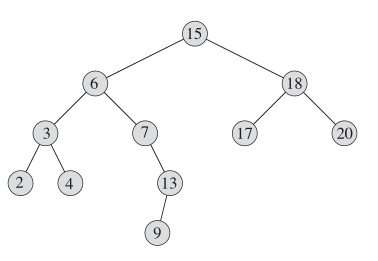
\includegraphics[scale = 0.7]{bst_example}\\
  \caption{Binary search tree example}\label{fig.bst.example}
\end{figure}

On the other hand, as Exercise 12.2-6 asks you to show, \\
if the right subtree of node is empty and $x$ has a successor $y$, then $y$ is the lowest ancestor of $x$ whose left child is also an ancestor of $x$. In Figure \ref{fig.bst.example}, the successor of the node with key 13 is the node with key 15. T\textbf{o find $y$, we simply go up the tree from $x$ until we encounter a node that is the left child of its parent}; this is accomplished by lines 3-7 of TREE-SUCCESSOR.

Tree-Predecessor is symmetric to Tree-Successor, both run in time $O(h)$

\subsection{Insertion and deletion}
\textbf{Insertion}\\
\begin{verbatim}
TREE-INSERT(T, z)
1  y ← NIL // 这个初始化时必须的, 因为当x一开始就是nil时, 就直接在line 9 对y==nil 进行判断
2  x ← root[T]
3  while x neq NIL
4      do y ← x
5         if key[z] < key[x]
6            then x ← left[x]
7            else x ← right[x]
8  p[z] ← y
9  if y = NIL
10     then root[T] ← z  # Tree T was empty
11     else if key[z] < key[y]
12             then left[y] ← z
13             else right[y] ← z
\end{verbatim}

\noindent line 4: 将$x$保存下来, 是因为while循环结束的时候, $x=nil$, 也就是现在$x$是叶子节点的子节点, 这个时候, $x$的parent就是一个叶子节点, 也就是说$y$是一个叶子节点, 而$z$ 将要成为$y$的一个子节点.\\
如果我们不把x的parent 保存下来, 一旦我们走到了一个leaf 处, 我们就没有办法把$z$ 放置到我们已经找到的位置.

\bigskip
\textbf{Deletion}\\
3 cases:\\
1, if z has \textbf{no children},见图\ref{fig.bst.deletion.case.1}, 直接删除掉z 就行了

\begin{figure}[htbp]
  \centering
  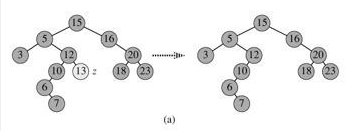
\includegraphics[scale = 0.7]{bst_deletion_case1}\\
  \caption{Case 1 of deletion}\label{fig.bst.deletion.case.1}
\end{figure}
%% figure:BST_delete_no_children\\

2, if $z$ has only \textbf{a single child}, 见图\ref{fig.bst.deletion.case.2},那么删除$z$, 将$z$ 的父节点与此孩子节点(子树) 关联就可以了
\begin{figure}[htbp]
  \centering
  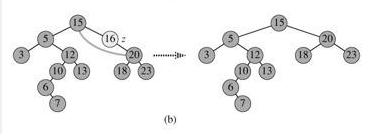
\includegraphics[scale = 0.7]{bst_deletion_case2}\\
  \caption{Case 2 of deletion}\label{fig.bst.deletion.case.2}
\end{figure}
%% figure: BST_delete_one_child

3, if $z$ has \textbf{two children},见图\ref{fig.bst.deletion.case.3}, 删除掉$z$ 的后继, 然后用$z$的后继来替代$z$\\
因为只有将$z$ 的后继放在$z$的位置, 才能够保持BST 的性质,$z$ 的后继由于是在$z$ 的右子树中的节点, 所以是大于$z$的左子树中所有的节点; 同时后继是右子树中最小的节点, 所以将这个后继挪到$z$的位置后, 是小于右子树中的所有节点\\
%% figure: BST_delete_two_children
\begin{figure}[htbp]
  \centering
  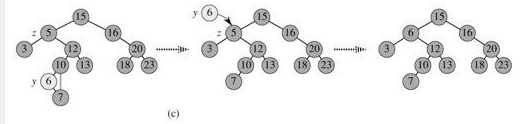
\includegraphics[scale = 0.7]{bst_deletion_case3}\\
  \caption{Case 3 of deletion}\label{fig.bst.deletion.case.3}
\end{figure}

我们可以将case 3 化为case 1和case 2两种已经解决的情况, 我们可以任意选取一个$z$的子树, 从底部开始, 把这个子树上所有的节点, 一个一个从树上摘下来, 存着, 然后$z$ 就成为一个只有一颗子树的节点, 然后就适用case 2. 删除完$z$ 后, 再把存着的那些节点重新插入到树上, 就完成了. 这个方法虽然有点笨, 但是确实是可行的.

其他办法: 要想不影响树的特性,那么最简单的想法是如果能只动$z$以及$z$以下的节点,那么树的其它部分肯定是OK的.那只要处理$z$以及$z$的子树就行了.想想,如果能在子树中找一个节点来替代$z$的位置,并保证新的子树也是满足二叉查找树要求的,这样改动量可能就比较小了.那么找哪个节点来代替它呢?当然是键值最接近X的,这样二叉树的特征就比较容易保持嘛.键值最接近$z$的,上面已经说过了,就是直接前趋和直接后继.正好,对于有两个子树的$z$来说,它的直接前趋和直接后继都是在它的子树中的,分别是左子树的最大值,右子树的最小值.而且,从子树中取下这两个节点(取下来干嘛?代替需要删除的X节点呗),也是比较容易的,因为"最大""最小"值节点,最多拥有不超过一个子节点(不然它绝对不够格做最大或最小).而没有子节点和只有一个子节点的节点删除,是我们已经会啦~~~.好,那么就\textbf{取前趋或后继就来代替需要删除的节点},问题就解决了.

\todo{这个代码不知道为什么不分三种情况来写, 非要写在一起, 看的就头疼, 还没有看懂}
\begin{verbatim}
TREE-DELETE(T, z)
1  if left[z] = NIL or right[z] = NIL
2      then y ← z
3      else y ← TREE-SUCCESSOR(z) //也可以用predeccessor
4  if left[y] neq NIL
5      then x ← left[y]
6      else x ← right[y]
7  if x neq NIL
8      then p[x] ← p[y]
9  if p[y] = NIL
10      then root[T] ← x
11      else if y = left[p[y]]
12              then left[p[y]] ← x
13              else right[p[y]] ← x
14  if y neq z
15      then key[z] ← key[y]
16           copy y's satellite data into z
17  return y
\end{verbatim}

\subsection{Randomly built binary search trees}
exponential height

\section{Red-Black Tress}
\noindent balanced search tree\\
$O(\lg n)$ height

\noindent Examples:\\
AVL trees\\
2-3 trees\\
2-3-4 trees\\
B-trees\\
Red-Black trees\\
Skip lists\\
Treaps

\subsection{Properties of red-black trees}
Red-black trees are one of many search-tree schemes that are "balanced" in order to guarantee that basic dynamic-set operations take $O(\lg n)$ time in the worst case.

\textbf{red-black properties}:
\begin{enumerate}
\item Every node is either red or black.
\item The root is black.
\item Every leaf ($NIL$) is black.
\item If a node is red, then both its children are black.
\item For each node, all simple paths from the node to descendant leaves contain the same number of black nodes.
\end{enumerate}

4 说明red 的parent 必须是black, 也就是说不能出现连续的两个red,\\
同时也说明at least half the nodes on any simple path from the root to a leaf, not including the root, must be black.

$bh(x)$: black height of $x$, 不包括$x$ 节点, 但包括叶节点$T.nil$

we use the one sentinel $T:nil$ to represent all the NILs—all leaves and the root's parent for saving space.
\begin{figure}[htbp]
  \centering
  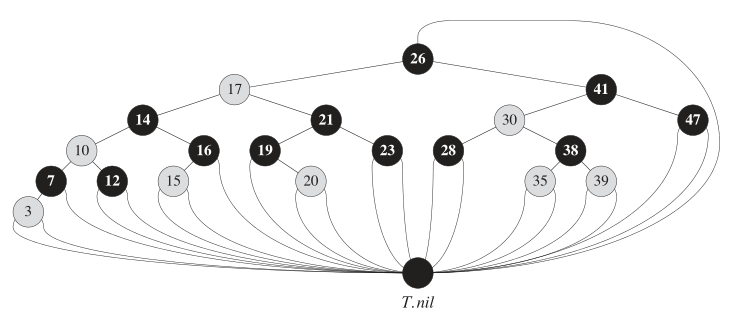
\includegraphics[scale = 0.7]{red_black_tree_presentation}\\
  \caption{Presentation of red black tree}\label{fig.rbt.presentation}
\end{figure}

在实际适用中, 为了方便, 我们有时不将$nil$ 画出.

\noindent \underline{Lemma}: A red-black tree with n internal nodes has height at most $2\lg(n+1)$.\\
\underline{Proof}: We start by showing that the subtree rooted at any node $x$ contains at least\\
$2^{bh(x)} - 1$ internal nodes. 这个用数学归纳法证明\\
To complete the proof of the lemma, let h be the height of the tree.\\
the black-height of the root must be at least $h/2$; thus,\\
$n \geq 2^{h/2} - 1 \Rightarrow h \leq 2 \lg(n+1)$\\

Although the algorithms TREE-INSERT and TREE-DELETE from Chapter 12 run in $O(\lg n)$ time\\
When given a red-black tree as input, they do not directly support the dynamic-set operations INSERT and DELETE, since they do not guarantee that the modified binary search tree will be a red-black tree. 后面会讲到

\subsection{Rotations}
A local operation in a search tree that preserves the binary-search-tree property
\begin{figure}[htbp]
  \centering
  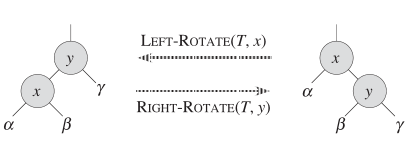
\includegraphics[scale = 0.7]{red_black_tree_rotation}\\
  \caption{Rotation in a search tree}\label{fig.rbt.rotation}
\end{figure}
tree rotation 对, 中序遍历没有影响

\begin{verbatim}
LEFT-ROTATE(T, x)
    y=x.right //set y
    x.right=y.left //turn y's left subtree into x's right subtree
    if y.left != T.nil
        y.left.p = x
    y.p = x.p
    if x.p == T.nil //link x's parent to y
        T.root = y
    elseif x == x.p.left
        x.p.left = y
    else x.p.right =y
    y.left = x //put x on y's left
    x.p = y
\end{verbatim}
\begin{figure}[htbp]
  \centering
  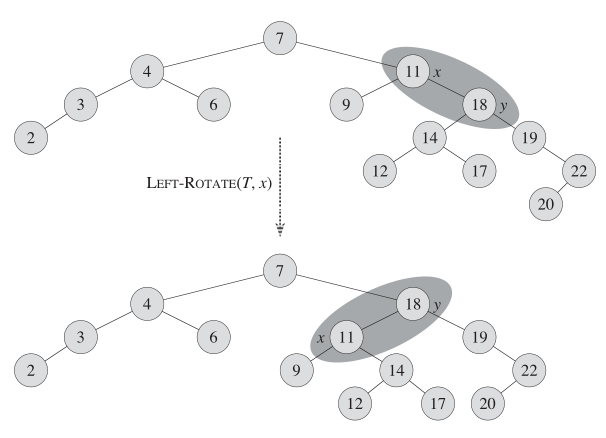
\includegraphics[scale = 0.7]{red_black_tree_rotation_example}\\
  \caption{Rotation example of a red black tree}\label{fig.rbt.rotation.example}
\end{figure}

\subsection{Insertion}
当我们insert 的时候, 我们总是把新的node color red, 因为如果color black, 那么distance(black height) 会成为棘手的问题, 相对于red-red clash而言

当进入到case 3, 表示就结束了\\
当进入到case 2时, 说明很快就会进入case 3, 所以也表示结束\\
所以在计算时间的时候, 我们只需要考虑case 1\\
在case 1的情形里, 每次都会将violation 往上移动two generations, 而树的高度$h<=2\lg(n+1)$, 所以情形一的循环次数最多为$\lg(n+1)$\\
所以最终是$\lg n$ time
\begin{verbatim}
RB-Insert(T,x):
    Tree-Insert(T,x)
    color[x] = red
    while x != root[T] or color[x]=red
    //当x 是根节点或者x是black node(不会有violation), 循环结束
        if p[x]=left[p[p[x]]] //A 类, A 与B是对称的, B: p[x]=right[p[p[x]]]
            y=right[p[p[x]]] //y is x's uncle
            if color[y]=red //y is red
                then <case 1>
            else if x=right[p[x]] //bad side
                    then <case 2>
                <case 3>  //good side,这里不用else, 因为case 2也会进入case 3
        else (same as catogory A with "right" and "left" exchanged) //B
    color[root[T]]=black //改变root的color 对distance 没有影响
\end{verbatim}

\subsection{Deletion}

\begin{verbatim}
RB-DELETE(T, z)
 1 if left[z] = nil[T] or right[z] = nil[T]
 2    then y ← z
 3    else y ← TREE-SUCCESSOR(z)// y is the realDelNode
 4 if left[y] neq nil[T] //if y has no children, x = nil
 5    then x ← left[y]
 6    else x ← right[y]
 7 p[x] ← p[y]
 8 if p[y] = nil[T]
 9    then root[T] ← x
10    else if y = left[p[y]]
11            then left[p[y]] ← x
12            else right[p[y]] ← x
13 if y 3neq z
14    then key[z] ← key[y]
15         copy y's satellite data into z
16 if color[y] = BLACK //if red, no need to fix up
17    then RB-DELETE-FIXUP(T, x)
18 return y

RB-DELETE-FIXUP(T, x)
 1 while x neq root[T] and color[x] = BLACK
 2     do if x = left[p[x]]
 3           then w ← right[p[x]]
 4                if color[w] = RED
 5                   then color[w] ← BLACK                        \\  Case 1
 6                        color[p[x]] ← RED                       \\  Case 1
 7                        LEFT-ROTATE(T, p[x])                    \\  Case 1
 8                        w ← right[p[x]]                         \\  Case 1
 9                if color[left[w]] = BLACK and color[right[w]] = BLACK
10                   then color[w] ← RED                          \\  Case 2
11                        x =p[x]                                  \\  Case 2
12                   else if color[right[w]] = BLACK
13                           then color[left[w]] ← BLACK          \\  Case 3
14                                color[w] ← RED                  \\  Case 3
15                                RIGHT-ROTATE(T, w)              \\  Case 3
16                                w ← right[p[x]]                 \\  Case 3
17                         color[w] ← color[p[x]]                 \\  Case 4
18                         color[p[x]] ← BLACK                    \\  Case 4
19                         color[right[w]] ← BLACK                \\  Case 4
20                         LEFT-ROTATE(T, p[x])                   \\  Case 4
21                         x ← root[T]                            \\  Case 4
22        else (same as then clause with "right" and "left" exchanged)
23 color[x] ← BLACK
\end{verbatim}

\textbf{Within the while loop, $x$ always points to a nonroot doubly black node}

\textbf{Case 1: $x$'s sibling w is red}\ \ See Figure \ref{fig.rbt.deletion.case1}\\
\begin{figure}[htbp]
  \centering
  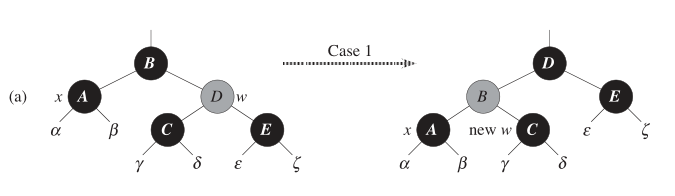
\includegraphics[scale = 0.7]{red_black_tree_deletion_case1}\\
  \caption{Case 1 for the deletion in a red black tree}\label{fig.rbt.deletion.case1}
\end{figure}
Case 1 (lines 5–8 of RB-DELETE-FIXUP and Figure \ref{fig.rbt.deletion.case1} occurs when node $w$, the sibling of node $x$, is red. \\
Since $w$ must have black children, we can switch the colors of $w$ and $x:p$ and then perform a left-rotation on $x:p$ without violating any of the red-black properties. The new sibling of x, which is one of $w$'s children prior to the rotation, is now black, and thus we have converted case $1$ into case $2$, $3$, or $4$.\\
Cases 2, 3, and 4 occur when node $w$ is black; they are distinguished by the colors of $w$'s children.

\textbf{Case 2: $x$'s sibling $w$ is black, and both of $w$'s children are black}\ \ See Figure \ref{fig.rbt.deletion.case2}\\
\begin{figure}[htbp]
  \centering
  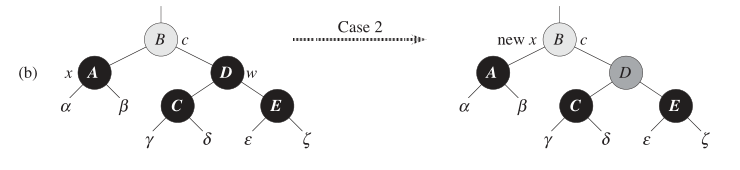
\includegraphics[scale = 0.7]{red_black_tree_deletion_case2}\\
  \caption{Case 2 for the deletion in a red black tree}\label{fig.rbt.deletion.case2}
\end{figure}
In case 2 (lines 10–11 of RB-DELETE-FIXUP and Figure \ref{fig.rbt.deletion.case2}), both of $w$'s children are black. Since $w$ is also black, we take one black off both $x$ and w, leaving $x$ with only one black and leaving $w$ red. To compensate for removing one black from $x$ and w, we would like to add an extra black to $x:p$, which was originally either red or black. We do so by repeating the while loop with $x:p$ as the new node $x$. Observe that if we enter case 2 through case 1, the new node $x$ is red-and-black, since the original $x:p$ was red. Hence, the value $c$ of the color attribute of the new node $x$ is RED, and the loop terminates when it tests the loop condition. We then color the new node $x$ (singly) black in line 23.

\textbf{Case 3: $x$'s sibling $w$ is black, $w$'s left child is red, and $w$'s right child is black}\ \ See Figure \ref{fig.rbt.deletion.case3}\\
\begin{figure}[htbp]
  \centering
  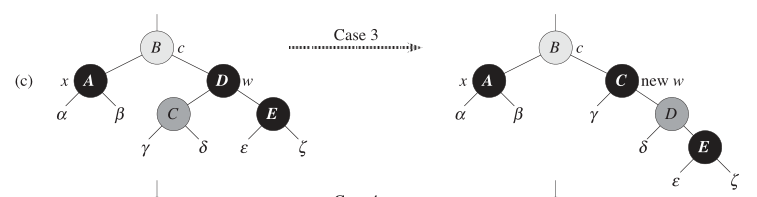
\includegraphics[scale = 0.7]{red_black_tree_deletion_case3}\\
  \caption{Case 3 for the deletion in a red black tree}\label{fig.rbt.deletion.case3}
\end{figure}
Case 3 (lines 13–16 and Figure \ref{fig.rbt.deletion.case3}) occurs when $w$ is black, its left child is red, and its right child is black. \\
We can switch the colors of $w$ and its left child w:left and then perform a right rotation on $w$ without violating any of the red-black properties. The new sibling $w$ of $x$ is now a black node with a red right child, and thus we have transformed case 3 into case 4.

\textbf{Case 4: $x$'s sibling $w$ is black, and $w$'s right child is red}\ \ See Figure \ref{fig.rbt.deletion.case4}\\
\begin{figure}[htbp]
  \centering
  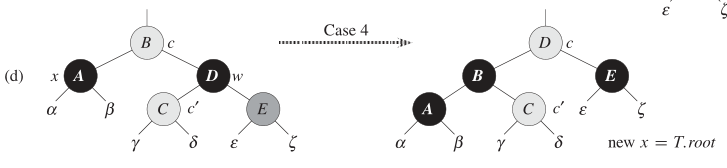
\includegraphics[scale = 0.7]{red_black_tree_deletion_case4}\\
  \caption{Case 4 for the deletion in a red black tree}\label{fig.rbt.deletion.case4}
\end{figure}
Case 4 (lines 17–21 and Figure \ref{fig.rbt.deletion.case4}) occurs when node $x$'s sibling $w$ is black and $w$'s right child is red. By making some color changes and performing a left rotation on $x:p$, we can remove the extra black on x, making it singly black, without violating any of the red-black properties. Setting $x$ to be the root causes the while loop to terminate when it tests the loop condition.

\subsection{Analysis}
height of a red-black tree of n nodes is $O(\lg n)$\\
the total cost of the procedure without the call to RB-DELETE-FIXUP takes $O(\lg n)$ time.\\
Within RB-DELETE-FIXUP, each of \textbf{cases $1$, $3$, and $4$ lead to termination} after performing a constant number of color changes and at most three rotations.\\
Case 2 is the only case in which the while \underline{loop can be repeated}, and then the pointer $x$ moves up the tree at most $O(\lg n)$ times, performing no rotations. Thus, the procedure RB-DELETE-FIXUP takes $O(\lg n)$ time and performs at most three rotations, and the overall time for RB-DELETE is therefore also $O(\lg n)$

\section{Augmenting data structures}
\subsection{Dynamic order statistics}
\noindent $select(x, i)$ return $i$\textsuperscript{th} smallest element in the subtree rooted at $x$\\
$rank(x)$ return the rank of a given element in the total ordering of the set\\
$size[x]$ which is the number of nodes in the subtree rooted at $x$.
\begin{figure}[htbp]
  \centering
  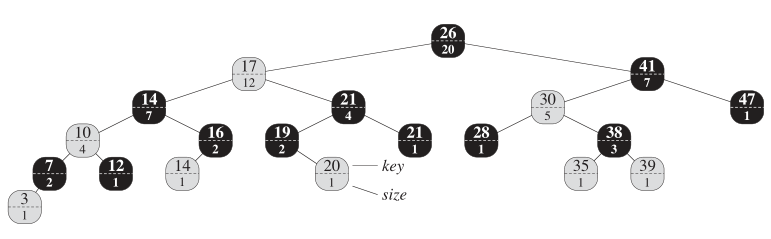
\includegraphics[scale =0.7]{order_statistics_tree}\\
  \caption{An order statistics tree}\label{fig.order_statistics_tree}
\end{figure}

\bigskip
An \textbf{order-statistic tree} $T$ is simply a red-black tree with additional information (size) stored in each node.\\
$size[x] = size[left[x]] + size[right[x]] + 1$\\
$size[nil] = 0$

\bigskip
在order-statistic tree中, 可以有相同的keys, 但是这样我们就需要重新定义一下rank\\
\textbf{rank}: the position at which it would be printed in an inorder walk of the tree.

\begin{verbatim}
OS-select(x, i)
    r = size[left[x]] + 1
    if i = r
        return x
    else if i<r
        return OS-select(left[x], i)
    else return OS-select(right[x], i - r)
\end{verbatim}

$O(\lg n)$ time

\begin{verbatim}
OS-RANK(T,x)
    r = size[left[x]] + 1
    y = x
    while y != root[T]
        if y = right[p[y]]
            r = r + size[left[p[y]]] + 1
        y = p[y]
    return r
\end{verbatim}

$O(\lg n)$ time

maintaining subtree sizes\\
刚开始的时候, 为一个干净的红黑树添加size, 需要$O(\lg n)$ time\\
在insert 和 delete 操作的时候, update size 是$O(1)$ 的操作, 因此insert 和 delete 仍然是 $O(\lg n)$ 的操作

\subsection{How to augment a data structure}
\underline{Theorem} 14.1 (\textbf{Augmenting a red-black tree})\\
Let f be an attribute that augments a red-black tree $T$ of $n$ nodes, and suppose that the value of $f$ for each node $x$ depends on only the information in nodes $x$, $x:left$, and $x:right$, possibly including $x:left:f$ and $x:right:f$. Then, we can maintain the values of $f$ in all nodes of $T$ during insertion and deletion without asymptotically affecting the $O(\lg n)$ performance of these operations.

\subsection{Interval tree}
这里我们研究的都是闭区间\\
Given a query interval, we can then quickly find an interval in the set that overlaps it

\textbf{interval trichotomy}\\
Any two intervals i and i' satisfy the interval trichotomy; that is, exactly one of the following three properties holds:
\begin{enumerate}
\item $i$ and $i'$ overlap,
\item $i$ is to the left of $i'$ (i.e., $high[i] < low[i']$),
\item $i$ is to the right of $i'$ (i.e., $high[i'] < low[i]$).
\end{enumerate}

we say that intervals $a$ and $b$ \textbf{overlap} if $a \cap b \neq \varnothing$ (Tex 中空集的表示方法),\\
that is if $low[a] \leq high[b]$ and $low[b] \leq high[a]$

Aninterval tree isared-black tree that maintains adynamic setof elements, with each element $x$ containing an interval $x:int$.

\noindent INTERVAL-INSERT(T, x)\\
INTERVAL-DELETE(T, x)\\
INTERVAL-SEARCH(T, i): returns a pointer to an element $x$ in the interval tree $T$ such that $int[x]$ overlaps interval $i$, or a pointer to the sentinel $nil[T]$ if no such element is in the set.
\begin{figure}[htbp]
  \centering
  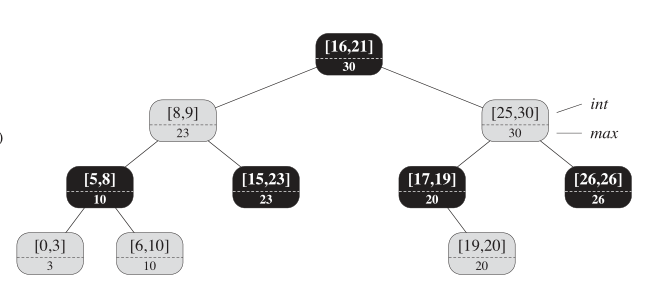
\includegraphics[scale =0.7]{interval_tree}\\
  \caption{An interval tree}\label{fig.interval_tree}
\end{figure}

\bigskip
\textbf{Underlying data structure}\\
We choose a red-black tree in which each node $x$ contains an interval $x:int$ and the key of $x$ is the low endpoint\\
\textbf{Additional information}\\
In addition to the intervals themselves, each node $x$ contains a value $x:max$, which is the maximum value of any interval endpoint stored in the subtree rooted at $x$\\
\textbf{Maintaining the information}\\
We must verify that insertion and deletion take $O(\lg n)$ time on an interval tree of n nodes. We can determine $x:max$ given interval $x:int$ and the max values of node $x's$ children:\\
$max[x] = max(high[int[x]], max[left[x]], max[right[x]])$\\
\textbf{Developing new operations}
\begin{verbatim}
INTERVAL-SEARCH(T, i)
    x = root[T]
    while x != nil[T] and i does not overlap int[x]
        if left[x] != nil[T] and max[left[x]] >= low[i]
            x = left[x]
        else x = right[x]
    return x
\end{verbatim}
也可以写成递归的形式, tail recursive call

\bigskip
\noindent list all overlapping intervals:\\
if $I$ have $k$ overlaps, then the time is $O(k\lg n)$\\
if $I$ search the second time, I get the same interval, so when I find one, delete it, and search agagin\\
output sensitive, 运行时间取决于输出结果

\bigskip
\noindent \underline{Theorem}: let $L = {i \in left[x]}, R = {i \in right[x]}$\\
1.if search goes right, then ${i' \in L, i' \eqnote{overlaps} i} = \varnothing$\\
2.if search goes left, then ${i' \in L, i' \eqnote{overlaps} i} = \varnothing => {i' \in R, i' \eqnote{overlaps} i} = \varnothing$\\
对于2. search goes left, 如果这时在左边没有找到overlaps, 那么我们也不可能在右边找到

\bigskip
segment tree

\section{Skip list}
dynamic search structure \\
efficient, randomized, simple\\
$O(\lg n)$ in expectation with high probability($\simeq 1 - 1/(n^{\alpha})$)

\bigskip
\noindent (sorted linked list)\\
$2$ sorted linked lists

\bigskip
\noindent L2: stores all elements\\
L1: stores some elements

\section{Dynamic programming}
optimal sub structure\\
a very powerful algorithmic paradigm in which a problem is solved by \textbf{identifying a collection of subproblems and tackling them one by one, smallest first, using the answers to small problems to help figure out larger ones, until the whole lot of them is solved}. \\
In dynamic programming we are not given a dag; the dag is implicit. Its nodes are the subproblems we define, and its edges are the dependencies between the subproblems: if to solve subproblem $B$ we need the answer to subproblem $A$, then there is a (conceptual) edge from $A$ to $B$. In this case, $A$ is thought of as a smaller subproblem than $B$\ ---\ and it will always be smaller, in an obvious sense.

Dynamic programming is effective when a given sub problem may arise from more than one partial set of choices; \textbf{the key technique is to store the solution to each such sub problem in case it should reappear}.\\
A dynamic programming algorithm will \underline{examine all possible ways} to solve the problem and will pick the best solution. Therefore, we can roughly think of dynamic programming as an intelligent, \underline{brute-force method} that enables us to go through all possible solutions to pick the best one. If the scope of the problem is such that going through all possible solutions is possible and fast enough, dynamic programming guarantees finding the optimal solution. The alternatives are many, such as using a greedy algorithm, which picks the best possible choice "at any possible branch in the road". While a \underline{greedy algorithm} does not guarantee the optimal solution, it is faster. Fortunately, some greedy algorithms (such as minimum spanning trees) are proven to lead to the optimal solution.

\underline{For example}, let's say that you have to get from point $A$ to point $B$ as fast as possible, in a given city, during rush hour. \\
A dynamic programming algorithm will look into the entire traffic report, looking into all possible combinations of roads you might take, and will only then tell you which way is the fastest. Of course, you might have to wait for a while until the algorithm finishes, and only then can you start driving. The path you will take will be the fastest one (assuming that nothing changed in the external environment). On the other hand, a greedy algorithm will start you driving immediately and will pick the road that looks the fastest at every intersection. \\
As you can imagine, this strategy might not lead to the fastest arrival time, since you might take some "easy" streets and then find yourself hopelessly stuck in a traffic jam.\\

\noindent
\textbf{Greedy algorithms}: make each choice in a locally optimal manner.\\
\textbf{Amortized analysis}: Instead of bounding the cost of the sequence of operations by bounding the actual cost of each operation separately, an amortized analysis provides a bound on the actual cost of the entire sequence. One advantage of this approach is that although some operations might be expensive, many others might be cheap.

We typically apply dynamic programming to \textbf{optimization problems}. Such problems can have many possible solutions. Each solution has a value, and we wish to \textbf{find a solution with the optimal (minimum or maximum) value}. We call such a solution an optimal solution to the problem, as opposed to the optimal solution, since there may be several solutions that achieve the optimal value.

When developing a dynamic-programming algorithm, we follow a sequence of four steps:
\begin{enumerate}
\item Characterize the structure of an optimal solution.
\item Recursively define the value of an optimal solution.
\item Compute the value of an optimal solution, typically in a bottom-up fashion.
\item Construct an optimal solution from computed information
\end{enumerate}

\subsection{Assembly-line scheduling}
 一个车间有2 条生产线, each assembly line with n stations, numbered by $j = 1, 2, 3, …,n$\\
$S_{i,j}$ the $j$\textsuperscript{th} station on assembly line $i$ ($i = 1$ or $2$)\\
$j$\textsuperscript{th} station on line 1 and $j$\textsuperscript{th} station on line 2 have the same function, but the time required varies.\\
assembly time on line $i$ at station $j$ is $a_{i , j}$\\
transfer time from line $i$ at station $j$ is $t_{i,j}$, $j = 1,2, … n-1$\\
enter time: $e_i$\\
exit time: $x_i$

\textbf{Step 1: the structure of the fastest way through the factory}\\
let us consider the fastest possible way for a chassis to get from the starting point through station $S_{1, j}$\\
if $j =1$, there is only one way\\
if $j=2,3,..n-1$, two ways, come from station $S_{1, j-1}$ and then directly to station $S_{1,j}$\\
or come from station $S_{2, j-1}$ and be transferred to station $S_{1, j}$

\textbf{Step 2: a recursive solution}\\
let $f_i[j]$ denote the fastest possible way to get a chassis from the starting point through station $S_{i,j}$\\
我们最终要求的是: 让一个chassis 最快速的通过这个组装线, we note it as $f^*$\\
$f^* = min(f_1[n] + x_1, f_2[n] + x_2)$

$$
\begin{aligned}
& f_1[1] = e_1 + a_{1,1}\\
& f_1[j] = min(f_1[j-1] + a_{1,j}, f_2[j-1] + t_{2, j-1} + a_{1, j} \si j \geq 2\\
& \\
& f_2[1] = e_2 + a_{2,1}\\
& f_2[j] = min(f_2[j-1] + a_{2,j}, f_1[j-1] + t_{1, j-1} + a_{2, j} \si j \geq 2\\
\end{aligned}
$$

\noindent
the $f_i[j]$ values give the values of optimal solutions to sub problems. To help us keep track of how to construct an optimal solution, let us define $l_i[j]$ to be the line number $i$($1$ or $2$), whose $j$\textsuperscript{th} station is used through the station $S_{i,j}$. here, $j=2,3,… n$\\
$l^*$ the line whose station $n$ is used\\
For example: $l^* = 1$, means we use station $S_{1,6}$\\
now we look at $l_1[6]$, which is $2$, means we use station $S_{2,5}$\\
now we look at $l_2[5]$, which is $2$, means we use station $S_{2,4}$\\
now we look at $l_2[4]$, which is $1$, means we use station $S_{1,3}$\\
now we look at $l_1[3]$, which is $2$, means we use station $S_{2,2}$\\
now we look at $l_2[2]$, which is $1$, means we use station $S_{1,1}$\\
这样我们就能够逆序追踪我们的最优解

\textbf{Step 3: Computing the fastest times}\\
如果直接计算, 类似于Fibonacci 数列的直接计算, 需要exponential time,\\
但是也同样类似于Fibonacci 数列, 后面的值只是取决于前面的值, 所以我们如果把前面已经计算出来的值保存下来, 每个$f$ 的计算都只需要常数的时间

\begin{verbatim}
FASTEST-WAY(a,t,e,x,n)
    f_1[1] = e_1 + a_{1,1}
    f_2[1] = e_2 + a_{2,1}
    for j = 2 to n:
        if f_1[j-1] + a_{1,j} <= f_2[j-1] + t_{2,j-1} + a_{1,j}
            f_1[j] = f_1[j-1] + a_{1,j}
            l_1[j] = 1
        else
            f_1[j] = f_2[j-1] + t_{2,j-1} + a_{1,j}
            l_1[j] = 2
        if f_2[j-1] + a_{2,j} <= f_1[j-1] + t_{1,j-1} + a_{2,j}
            f_2[j] = f_2[j-1] + a_{2,j}
            l_2[j] = 2
        else
            f_2[j] = f_1[j-1] + t_{1,j-1} + a_{2,j}
            l_2[j] = 1 //end for

    if f_1[n] + x_1 <= f_2[n] + x_2
        f^* = f_1[n] + x_1
        l^* =1
    else
        f^* = f_2[n] + x_2
        l^* =2
\end{verbatim}

\noindent
$\Omega(n)$ time

\textbf{Step 4: Constructing the fastest way through the factory}
\begin{verbatim}
PRINT-STATIONS(l,n)
    i = l^*
    print "line ",i,", station ",n
    for j = n downto 2
        i = l_i[j]
        print "line ",i,", station ",n
\end{verbatim}
这个打印是逆序的, 如果要正序输出, 可以采用recursive, 或者stack

\subsection{Longest common subsequence (LCS)}
Ex: longest common subsequence (LCS)
\begin{verbatim}
x : A B C B D A B
y : B D C A B A
\end{verbatim}
LCS: BDAB, BCAB, BCBA 都是长度为$4$, 没有长度为$5$

\bigskip
Analysis\\
check if a sequence is in $y:O(n), y$ is of length $n$\\
$2^m$ subsequences of $x$ ($x$ is of length $m$)\\
check all sub sequences of $x: O(n \cdot 2^m)$\\
exponential time = slow!

\bigskip
Simplification\\
1.look at the length of LCS(x,y)\\
2.Extend the alg to find LCS itself\\
Notation: $|s|$ denotes length of seq $s$\\
Strategy: consider \textbf{prefixs} of $x$ and $y$\\
Define $c[i,j] = |LCS(x[1… i], y[1…j])|$\\
Then, $c[m,n] = |LCS(x,y)|$\\
找出$c[i,j]$ 的通项公式

\bigskip
\underline{Theorem}:
$$
c[i,j] = c[i-1,j-1] + 1 if x[i] = y[j]
$$
$$
c[i,j] =max(c[i,j-1], c[i-1,j]) \eqnote{otherwise}
$$
\underline{Proof}:

\subsection{Fibonacci}
top-down approach
\begin{verbatim}
var m := map(0 → 0, 1 → 1)
   function fib(n)
       if map m does not contain key n
           m[n] := fib(n - 1) + fib(n - 2)
       return m[n]
\end{verbatim}
$O(n)$ time but requires $O(n)$ space
top-down approach 也可以减少空间的使用, 就是向bottom-up一样, 覆盖掉不用的值

\bigskip
bottom-up approach
\begin{verbatim}
function fib(n)
       if n = 0
           return 0
       var previousFib := 0, currentFib := 1
       else repeat n - 1 times  // loop is skipped if n=1
           var newFib := previousFib + currentFib
           previousFib := currentFib
           currentFib  := newFib
       return currentFib
\end{verbatim}
$O(n)$ time and requires $O(1)$ space\\
bottom-up 把previousFib 之前的都丢了, 所以可以减少空间的使用

\subsection{Optimal binary search trees}
might be compared with \textbf{Huffman trees}, which similarly seek to \textbf{place frequently used items near the root in order to produce a dense information encoding}; however, Huffman trees only store data elements in leaves and these elements need not be ordered.

\subsection{Common subproblems}
Finding the right subproblem takes creativity and experimentation. But there are a few standard choices that seem to arise repeatedly in dynamic programming.

i.The input is $x_1 ,x_2 ,\ldots ,x_n$ and a subproblem is $x_1,x_2,\ldots,x_i$ .\\
The number of subproblems is therefore linear.

ii.The input is $x_1,\ldots,x_n$ , and $y_1 ,\ldots ,y_m$ . A subproblem is $x_1 ,\ldots ,x_i$ and $y_1 ,\ldots ,y_j$ .\\
The number of subproblems is $O(mn)$.

iii.The number of subproblems is $O(mn)$.\\
The number of subproblems is $O(n2)$.

iv.The input is a rooted tree. A subproblem is a rooted subtree.\\
If the tree has n nodes, how many subproblems are there? exponential

\section{贪婪算法和最小生成树}
A greed algorithm always makes the choice that looks best at the moment. That is, it makes a locally optimal choice in the hope that this choice will lead to a globally optimal solution.

Dynamic programming usually solves the sub problems bottom up, a greedy algorithm usually progresses in a top-down fashion, making one greedy choice after another, reducing each given problem instance to a smaller one.

\subsection{Greedy versus dynamic programming}
The 0-1 knapsack problem:\\
Insolvable by greedy strategy, solvable by dynamic programming\\
Unable to fill the knapsack to capacity, and the empty space lowers the effective value per pound.

The fractional knapsack problem:\\
Solvable by greedy strategy, compute the value per pound $v_1/w_i$ for each item, take as much as possible of the item with the greatest value per pound.

\subsection{Tree}
\noindent
Graph: $E = O(V^2) \Rightarrow \lg E = O(\lg V)$  //省略绝对值的写法\\
digraph: directed graph\\
connected $\Rightarrow |E| > |V| - 1$: there is a path from any vertex to any other vertex in the graph.

adjacency matrix邻接矩阵 $n \times n$ matrix\\
where $V={1,2, … n}$\\
$A[i,j] = 1 \si (i,j) \in E$\\
$A[i,j] = 0 \si (i,j) \not \in E$
\begin{figure}[htbp]
  \centering
  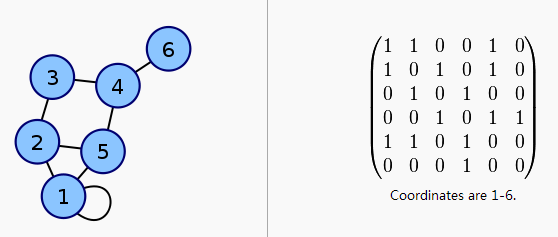
\includegraphics[scale = 0.7]{adjacency_matrix}\\
  \caption{Represent a graph with adjacency matrix}\label{fig.adjacency.matrix}
\end{figure}

Represent a graph with adjacency matrix, $O(V^2)$ storage $\Rightarrow$ dense representation\\
a complete graph, all elements are $1$

a sparse graph稀疏矩阵: 极端例子 a linked list
\begin{figure}[htbp]
  \centering
  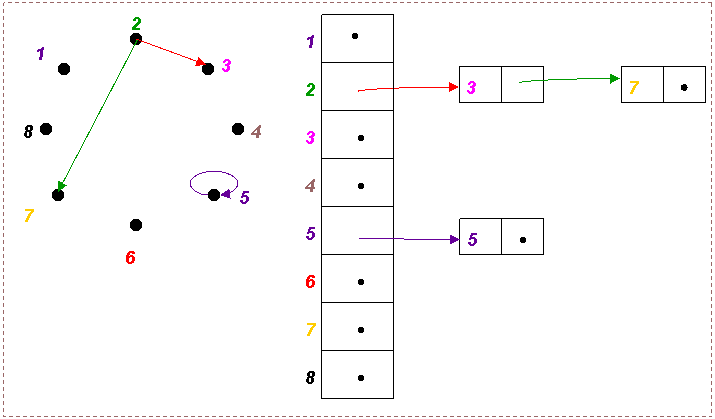
\includegraphics[scale = 0.6]{adjacency_list}\\
  \caption{Represent a graph with adjacency list}\label{fig.adjacency.list}
\end{figure}

Adjacency list\\
矩阵中每一行为1组成的一个list

\noindent
$|\mbox{Adj}[j]| =$ degree  if undirected graph\\
$|\mbox{Adj}[j]| =$ out degree  if directed graph

Handshaking Lemma (undirected graph)\\
$\sum_{v \in V} degree(v) = 2|E|$\\
每加入一条边, 这条边的两个顶点的degree 都增加$1$\\
For undirected graphs $\Rightarrow$ adjacency list uses $\Theta(V+E)$ storage

\subsection{Huffman code}
Huffman coding is a form of statistical coding.\\
Decoding: Once receiver has tree, it scans incoming bit stream, 0 means go left and 1 means go right.\\
Huffman coding is an entropy encoding algorithm used for lossless data compression.

\textbf{Huffman's paper: A method for the construction of minimum redundancy codes}

\textbf{Arithmetic coding and LZW coding}\\
\textbf{Linear time if input probabilities are sorted}

Uniform probability distribution and a number of members which is a power of two: Huffman coding is equivalent to simper binary block encoding, eg ASCII coding.

Shannon-Fano coding

A symbol with zero probability has zero contribution to the entropy.\\
$\lim_{p \to 0} p \cdot \log_{2} p = 0$

Entropy: the theoretical limit length established by Shannon.

A prefix code (sometimes called "prefix free codes") that is the bit string representing some particular symbol is never a prefix of the bit string representing another symbol.

\subsection{MST - Minimum spanning tress}
Distributed system\\
Input: connected, undirected graph $G=(V, E)$\\
$N: E \rightarrow R$ 权值\\
For simplicity, assume all edge weights are distinct $\Rightarrow N$ is injective\\
Output: A spanning tree $T$ (connects all vertexes) of minimum weight\\
	$W(T) = \sum_{(u, v) \in T} w(u, v)$ //$(u,v)$ is an edge

\begin{figure}[htbp]
  \centering
  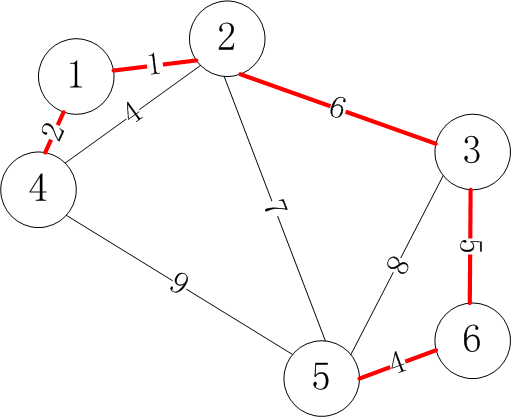
\includegraphics[scale = 0.5]{mst_result}\\
  \caption{红色是最小生成树的结果}\label{fig.mst.result}
\end{figure}

remove $(u, v)$ from $T$, then $T$ is partitioned into two sub trees $T_1$ and $T_2$\\

\noindent
\underline{Theorem}: $T_1$ is MST for $G_1 = (V_1, E_1)$ the sub graph of $G$ induced by vertexes in $T_1$\\
for $T_2$ the same thing\\
\underline{Proof}: cut and paste\\
$W(T) = W(u, v) + W(T_1) + W(T_2)$\\
if $\exists T'$ better than $T_1$ for $G_1$, then\\
overlapping sub problems? Yes\\
dynamic programming? Yes, but MST exhibits a better property $\Rightarrow$ greedy algorithm

\noindent
\underline{Theorem}: Let $T$ be MST of $G=(V, E)$, Suppose $(u,v)$ in $E$, least-weight edge connecting $A$ to $V-A$, then $(u,v)$ in $T$\\
\underline{Proof}: cut and paste

\section{Amortized Analysis}
\subsection{Incrementing a binary counter}
A k-bit binary counter that counts upward from $0$.\\
Use an array $A[0…k-1]$ of bits, where $A.length = k$, as the counter.\\
A binary number $x$ that is stored in the counter has its lowest-order bit in $A[0]$ and its highest-order bit in $A[1]$, so that $x=\sum_{i=0}^{k-1} A[i]*2^i$. Initially, $x = 0$
\begin{verbatim}
Increment(A)
    i = 0
    while i<A.length and A[i] == 1
        A[i] =0
        i = i + 1
    if i < A.length
        A[i] = 1
\end{verbatim}

A single execution of INCREMENT takes time $\Theta(k)$ in the worst case, in which array $A$ contains all $1$s. Thus, a sequence of $n$ INCREMENT operations on an initially zero counter takes time $O(nk)$ in the worst case.\\
We can tighten our analysis to yield a worst-case cost of $O(n)$ for a sequence of $n$ INCREMENT operations by observing that not all bits flip each time INCREMENT is called.\\
$A[0]$ does flip each time INCREMENT is called\\
$A[1]$, flips only every other time, flips $n/2$ times\\
Similarly, bit $A[2]$ flips only every fourth time, or $n/4$ times\\
bit $A[i]$ flips $n/(2^i)$ times in a sequence of $n$ INCREMENT operations on an initially zero counter.\\
For $i \geq k$, bit $A[i]$ does not exist, and so it cannot flip. The total number of flips in the sequence is thus
$$
\sum_{i=0}^{k-1}\lfloor \frac{n}{2^i} \rfloor
< n \sum_{i=0}^{\infty} \frac{1}{2^i}
= 2n
$$
The worst-case time for a sequence of $n$ INCREMENT operations on an initially zero counter is therefore $O(n)$. The average cost of each operation, and therefore the amortized cost per operation, is $O(n)/n = O(1)$
\subsection{Dynamic tables}
\begin{verbatim}
insert elements
     i	1	2	3	4	5	6	7	8	9 	10
size_i	1	2	4	4	8	8	8	8	16	16
cost_i	1	2	3	1	5	1	1	1	9 	1
\end{verbatim}

Cost of n inserts
$$
=\sum_{i=1}^n \mbox{cost}_i
=n+\sum_{j=0}^{\lfloor (\lg (n-1))\rfloor } 2^j
\leq 3n = \Theta(n)
$$
The average cost of a insert $= \Theta(n)/n=\Theta(1)$

\textbf{Amortized analysis}\\
Analyze a sequence of operations to show that average cost is small, even though 1 or serveral operations may be expensive\\
这里不涉及到概率分析

Types of amortized arguments\\
Aggregate (just saw)\\
accounting\\
potential

\subsection{Accounting method}
charge the $i$\textsuperscript{th} operation a fictitious amortized cost $c_i$ ($1$ pays for $1$ unit of operation)\\
fee is consumed to perform op\\
unused amount stored in bank for use in later ops

bank balance must not go negative:
$\sum_{i=1}^n \mbox{true-cost}_i \leq \sum_{i=1}^n \mbox{amortized-cost}_i$

\bigskip
Dynamic table\\
Charge $c_i = 3$\$ for $i$\textsuperscript{th} insert\\
\indent	1\$ pays for immediate insert\\
\indent	2\$ stored for table doubling\\
When table doubles\\
	\indent	1\$ moves recent item\\
	\indent	1\$ moves old item
\begin{verbatim}
0	0	0	0	2	2	2	2
\end{verbatim}
第五项插入时, 收取3\$, 其中1\$ 用于自己的插入, 剩下的2\$ 存入bank, 第$6, 7, 8$ 项插入时, 进行同样的操作, 这时银行刚好有8\$的存款\\
插入第$9$ 项时, table 需要double, 银行中剩余的8\$ 刚好可以支付原来$8$个elements 的移动到新table的花费
\begin{verbatim}
0	0	0	0	0	0	0	0	2
\end{verbatim}

Invariant bank balance $\geq 0$\\
$\sum_{i=1}^n \mbox{amortized-cost}_i =  3n$\\
实际上第一项可以只支付2\$, 从而可以省下1\$.

\subsection{Potential method}
Bank account viewed as potential energy of dynamic set

Framework
start with data structure $D_0$
op $i$ transforms $D_{i-1}$ to $D_{i}$

Define potential function\\
$\Phi: \{D\} \rightarrow R$ such that $\Phi(D_0) = 0$ and $\Phi(D) \geq 0$\\
Amortized cost $ac_i$ with respect $\Phi$ is\\
$ac_i = c_i + \Phi(D_i) - \Phi(D_{i-1})$\\
if $\Phi(D_i) - \Phi(D_{i-1})>0$ overcharge\\
if $\Phi(D_i) - \Phi(D_{i-1})<0$ undercharge
$$
\begin{aligned}
\sum_{i=0}^n ac_i
&= \sum_{i=0}^n (c_i + \Phi(D_i) - \Phi(D_{i-1}))
&= \sum_{i=0}^n c_i + \Phi(D_n) - \Phi(D_0)
&= \sum_{i=0}^n c_i + \Phi(D_n)
\end{aligned}
$$
我们需要$\sum_{i=0}^n ac_i \geq \sum_{i=0}^n c_i$, 所以应该保证$\Phi(D_n)\geq 0$, 但是实际上我们不知道应该怎样选择这样一个potential function, 所以我们通常保证$\Phi(D_i) \geq 0$

\textbf{Table doubling}\\
Define: $\Phi(D_i) = 2i – 2^{ceil(\lg i)}$\\
(Assume $2^{ceil(\lg 0)} = 0$)\\
Note: $\Phi(D_0) = 0$ and $\Phi(D_i) \geq 0$ (because $ceil(\lg i) = \lg i$ or $\lg i + 1$)\\
For example:
\begin{verbatim}
full	full	full	full	full	full		
\end{verbatim}
插入了$6$ 个, 此时 $\Phi = 2*6 – 2^{ceil(\lg 6)} = 12 – 8 =4$\\
如果我们用accounting method, 那么
\begin{verbatim}
0	0	0	0	2	2		
\end{verbatim}
此时bank balance 是$4$, 和上面的potential 一样\\
Amortized cost of $i$\textsuperscript{th} insert
$$
\begin{aligned}
ac_i
&= c_i +\Phi(D_i) - \Phi(D_{i-1})\\
&=
\left\{
  \begin{array}{ll}
		  i & \si i-1 \mbox{exact power of } 2\\
		  1 & \sinon
  \end{array}
\right.
+ (2i – 2^{ceil(\lg i)}) - (2(i-1) – 2^{ceil(\lg (i-1))})\\
&=
\left\{
  \begin{array}{ll}
		  i & \si i-1 \mbox{exact power of } 2\\
		  1 & \sinon
  \end{array}
\right.
+ 2 - 2^{ceil(\lg i)} + 2^{ceil(\lg (i-1))}
\end{aligned}
$$

Case 1: $i -1$ is exact power of $2$
$$
ac_i = i + 2 - 2^{ceil(\lg i)} + 2^{ceil(\lg (i-1))}
= i + 2 – 2^{\lg (i-1) + 1} + 2^{\lg (i-1)} = i + 2 – 2*(i-1) + (i-1) = 3
$$

Case 2: $i -1$ is not exact power of $2$\\
$ac_i = 1 + 2 - 2^{ceil(\lg i)} + 2^{ceil(\lg (i-1))} = 3$\\
$ceil(\lg i)$ 与$ceil(\lg (i-1)$ 是相等的\\

\textbf{Conclusions}\\
Amortized costs provide a clean abstraction for data structure performance.\\
Diff potential functions or accounting costs may yield diff bounds

\section{Advanced data structures}
Because disks operate much more slowly than random-access memory, we measure the performance of B-trees not only by how much computing time the dynamic-set operations consume but also by how many disk accesses they perform.\par
Fibonacci heaps are key components of some of the asymptotically fastest algorithms to date for graph problems.

Splay trees

\textbf{Persistent data structure}: a data structure that always preserves the previous version of itself when it is modified. Such data structures are effectively immutable, as their operations do not (visibly) update the structure in-place, but instead always yield a new updated structure. (A persistent data structure is not a data structure committed to persistent storage, such as a disk; this is a different and unrelated sense of the word "persistent.")\par
A data structure is partially persistent if all versions can be accessed but only the newest version can be modified. The data structure is fully persistent if every version can be both accessed and modified. If there is also a meld or merge operation that can create a new version from two previous versions, the data structure is called confluently persistent. Structures that are not persistent are called ephemeral.

Fusion trees

Exponential search trees

\section{B-Trees}
B-trees are similar to red-black trees (Chap-ter 13), but they are better at minimizing disk I/O operations. Many database systems use B-trees, or variants of B-trees, to store information.\\
B-tree nodes may have many children, from a few to thousands.\\
If an internal B-tree node x contains x.n keys, then x has x.n+1 children. The keys in node x serve as dividing points separating the range of keys handled by x into x.n + 1 sub ranges, each handled by one child of x.\\
In a typical B-tree application, the amount of data handled is so large that all the data do not fit into main memory at once. The B-tree algorithms copy selected pages from disk into main memory as needed and write back onto disk the pages that have changed. B-tree algorithms keep only a constant number of pages in main memory at any time; thus, the size of main memory does not limit the size of B-trees that can be handled.

B-tree algorithm depends primarily on the number of DISK-READ and DISK-WRITE operations, we typically want each to read or write as much information as possible. \todo{这一段话不懂, 多读取信息和节点的大小有什么关系, 读取信息是物理上的}Thus, a B-tree node is usually as large as a whole disk page, and this size limits the number of children a B-tree node can have.
\subsection{Definition of B-Trees}
\section{AVL tree}
\noindent
Self-balancing binary search tree

The heights of the two child subtrees of any node differ by at most one;

Time complexity in big $O$ notation
\begin{verbatim}
        Average  	Worst case
 Space	O(n)	       O(n)
Search	O(\log n)	O(\log n)
Insert	O(\log n)	O(\log n)
Delete	O(\log n)	O(\log n)
\end{verbatim}

Worst case is when right subtree has height  1 more than the left subtree for every node.

\noindent
$N_h$: min \# of nodes of height $h$\\
$N_h = 1+ N_{h-1} + N_{h-2}$\\
It looks like Fibonacci\\
$N_h > F_h = \frac{\phi^h}{\sqrt{5}}$ with $\phi = 1.618$  golden ratio\\
 $\frac{\phi^h}{\sqrt{5}} < n => h < c * \lg n$

\textbf{Insert}\\
1. simple BST insert\\
2. fix AVL property from changed node up

\textbf{AVL sort}\\
1. insert $n$ items - $\Theta(n\lg n)$\\
2. in-order traversal -$\Theta(n)$
\section{Graph}
We adopt a common notational convention: only inside asymptotic notation, such as $O$-notation, $\Theta$-notation, the symbol $V$ denotes $|V|$ and the symbol $E$ denotes $|E|$.

\noindent
The vertex set of a graph: $V[G]$\\
The edge set of a graph: $E[G]$

Sparse graph: $|E|$ is much less than $|V|^2$

\textbf{Breadth-first search: BFS}\\
Breadth-first search is so named because it expands the frontier between discovered and undiscovered vertices uniformly across the breadth of the frontier. That is, the algorithm discovers all vertices at distance $k$ from $s$ before discovering any vertex at distance $k+1$.

\bigskip
三种颜色的含义:\\
\textbf{White}: not having been discovered\\
\textbf{Gray}: frontier, discovered vertices that have not yet had their adjacency lists fully examined\\
\textbf{Black}: all its adjacency vertices have been examined

\noindent
$O(V+E)$ time

\bigskip
\textbf{Breadth-first trees}\\
The procedure BFS builds a breadth-first tree as it searches the graph, the tree is represented by the $\pi$ field in each vertex.\\
$G=(V, E)$ with source $s$\\
Predecessor subgraph of $G$ as $G\pi = (V\pi, E\pi)$, where\\
$V\pi = {v \in V: \pi[v] != NIL} {\cup s}$\\
$E\pi = {(\pi[v], v) : v \in V\pi - {s}}$

\section{最短路径算法}
Negative edge weight $\Rightarrow$ some shortest path may not exist.\\
Ex:\\
1.	图中出现了一个环, 而且这个环的总权值是负的negative cycle, 那么从u 到v的路径到达这个环时, 由于这个环的权值是负的, 它会永远地绕着这个环转下去, 使路径不断地变短\\
2.	$u$ 和$v$ 之间根本就没有路径

\textbf{optimal substructure}\\
a sub-path of a shortest path is shortest path.  // 用反证法 contradiction\\
Triangle inequality\\
$dist(u,v) \leq dist(u,x) + dist(x,v)$ //最短路径的定义\\
dist 表示最短路径

\textbf{Single source shortest path problem}\\
从源点$s$ 到所有其他点的最短路径\\
Assume all the edge weight are non-negative.\\
Idea: greedy

\subsection{Dijkstra's algorithm}
详细的可以看en wiki\\
a graph search algorithm that solves the single-source shortest path problem for a graph with non-negative edgepath costs, producing a shortest path tree. This algorithm is often used in routing and as a subroutine in other graph algorithms.\\
It picks the unvisited vertex with the lowest-distance, calculates the distance through it to each unvisited neighbor, and updates the neighbor's distance if smaller. Mark visited (set to red) when done with neighbors.

这里有一个图片(algo\_Dijkstra.gif),但是由于图片是gif 动态的, 无法放在这里
\begin{verbatim}
1  function Dijkstra(Graph, source):
2      for each vertex v in Graph:                                // Initializations
3          dist[v] := infinity ;     // Unknown distance function from source to v
5          previous[v] := undefined ;                // Previous node in optimal path
6      end for                                                    // from source
7
8      dist[source] := 0 ;                       // Distance from source to source
9      Q := the set of all nodes in Graph ; // All nodes in the graph are unoptimized –
                                                 //thus are in Q, priority queue
10    S: = empty set                  // no node optimized – thus S empty
11      while Q is not empty:                                      // The main loop
12          u := vertex in Q with smallest distance in dist[] ;    // Source node in first case
13          remove u from Q ;
14          if dist[u] = infinity:
15              break ;                                            // all remaining vertices are
16          end if                                                 // inaccessible from source
17          put u in S
18          for each neighbor v of u: //where v has not yet been removed from Q.
20              alt := dist[u] + dist_between(u, v) ;
21              if alt < dist[v]:                                  // Relax (u,v,a)
22                  dist[v] := alt ;
23                  previous[v] := u ;
24                  decrease-key v in Q;     // Reorder v in the Queue
                                       //因为v的距离被重新赋值了, 所以它在Q中的值也要相应地降低
25              end if
26          end for
27      end while
28      return dist;
29  end function
\end{verbatim}

Read the shortest path from source to target by reverse iteration
\begin{verbatim}
1  S := empty sequence
2  u := target
3  while previous[u] is defined:       // Construct the shortest path with a stack S
4      insert u at the beginning of S             // Push the vertex into the stack
5      u := previous[u]                           // Traverse from target to source
6  end while ;
\end{verbatim}

\noindent
Shortest path tree: the union of all shortest paths

breath first search: BFS 广度优先搜索\\
BFS 就是Dijkra\\

two changes\\
1. 不使用priority queue, 而是使用 FIFO queue\\
2. relax

\section{String matching}
The Rabin-Karp algorithm\\
String matching with finite automata\\
The Knuth-Morris-Pratt algorithm

\section{并行}
\noindent
parallel algorithms\\
dynamic multithreading\\
share memory, multicore
\begin{verbatim}
Ex: fib(n)
if n<2
    return n
x = spawn fib(n-1)
y = spawn fib(n-2)
sync
return (x+y)
\end{verbatim}
spawn: 衍生: Subroutine can execute at the same time with parent\\
Sync: wait until all children are done

\noindent
cashing
\section{Appendix}
\subsection{Summations}
\subsubsection{Approximation by integrals}
$$
\sum_{k=1}^n \frac{ 1}{k} \geq \int_1^{n+1}\frac{1}{x}dx = \ln(n+1)
$$

$$
\sum_{k=2}^n \frac{ 1}{k} \leq \int_1^{n}\frac{1}{x}dx = \ln n
$$
which yields the bound
$$
\sum_{k=1}^n \frac{ 1}{k} \leq \ln n + 1
$$

\subsection{Relations}
$v_0',v'_0$
A binary relation $R$ on two sets $A$ and $B$ is a subset of the Cartesian product$A \times B$
If $(a, b) \in R$, we sometimes write $a R b$. When we say that R is a binary relation on a set $A$, we mean that R is a subset of $A \times A$. For example, the "less than" relation on the natural numbers is the set $\{(a, b) : a, b$ in $N$ and $a < b\}$. An n-ary relation on sets $A_1, A_2,\ldots, A_n$ is a subset of $A_1 \times A_2 \times \cdots \times  A_n$.

A binary relation $R \subseteq A \times A$ is reflexive if
$a R b$ implies $b R a$ for all $a,b \in A$
\subsection{Probability}
$$
Pr(A\cap B)=\frac{Pr(A)*Pr(B \cap A)}{Pr(B)}
$$

$$
B=(B \cap A)\cup (B \cap \bar{A})
$$

$$
Pr(B)=Pr(B \cap A)+Pr(B \cap \bar{A})
=Pr(A)*Pr(B|A)+Pr(\bar{A})*Pr(B|\bar{A})
$$

$$
Pr(A\cap B)=\frac{Pr(A)*Pr(B \cap A)}{Pr(A)*Pr(B|A)+Pr(\bar{A})*Pr(B|\bar{A})}
$$

\end{document}
